\chapter{Organisation des sprints}
\section{Introduction}
Dans ce chapitre, nous allons présenter les sprints de notre projet. En premier lieu, nous allons spécifier le planning pour chaque sprint. Après, nous présenterons la modélisation statique et dynamique. Ensuite, nous allons détailler le développement du sprint. Et enfin, nous allons présenter le test, la revue du sprint et la rétrospective.

\section{Sprint 1: Tableaux de bords (du 13-02-2017 au 13-03-2017)}
Dans cette section, nous allons détailler la réalisation du sprint 1. En premier lieu, nous allons présenter la planification du sprint en présentant le but du sprint et le backlog sprint. Ensuite nous allons spécifier la modélisation statique et la modélisation dynamique. Puis, nous allons présenter le développement du sprint sous forme de capture d'écrans. Et nous finirons, enfin, avec le test, la revue et la rétrospective du sprint. 

\subsection{Sprint planning}
%But du sprint + backlog sprint%
Le but de ce sprint est de créer des tableaux de bords fonctionnels qui utilisent des données de notre base de données Jira. De ce fait, nous proposons le backlog sprint qui est représenté dans la table \ref{code56}.

\begin{longtable}{l}
\caption{Backlog du sprint1: "Tableaux de bords"} \label{code56} \\
\begin{tabular}{|c|l|l|l|}
\hline
\multicolumn{1}{|l|}{\textbf{User storyID}} & \textbf{User Story} & \textbf{Tâche ID} & \textbf{Tâche} \\ \hline
\multirow{3}{*}{1.1} & \multirow{3}{*}{\begin{tabular}[c]{@{}l@{}}En tant que membre, membre \\ senior ou chef d'équipe, je \\ souhaite pouvoir m'authentifier.\end{tabular}} & 1.1.1 & \begin{tabular}[c]{@{}l@{}}Réaliserles diagrammes UML \\ de la fonctionnalité \\ "s'authentifier".\end{tabular} \\ \cline{3-4} 
 &  & 1.1.2 & \begin{tabular}[c]{@{}l@{}}Développer la fonctionnalité \\ "s'authentifier".\end{tabular} \\ \cline{3-4} 
 &  & 1.1.3 & \begin{tabular}[c]{@{}l@{}}Tester la fonctionnalité \\ "s'authentifier".\end{tabular} \\ \hline
 \end{tabular} \\
\begin{tabular}{|c|l|l|l|}
\hline
\multicolumn{1}{|l|}{\textbf{User story ID}} & \textbf{User Story} & \textbf{Tâche ID} & \textbf{Tâche} \\ \hline
\multirow{3}{*}{3.1} & \multirow{3}{*}{\begin{tabular}[c]{@{}l@{}}En tant que chef d’équipe, \\ je souhaite pouvoir ajouter \\ un membre dans l’application.\end{tabular}} & 3.1.1 & \begin{tabular}[c]{@{}l@{}}Réaliser les diagrammes UML \\ de la fonctionnalité "Ajouter un \\ membre".\end{tabular} \\ \cline{3-4} 
 &  & 3.1.2 & \begin{tabular}[c]{@{}l@{}}Développer la fonctionnalité \\"Ajouter un membre".\end{tabular} \\ \cline{3-4} 
 &  & 3.1.3 & \begin{tabular}[c]{@{}l@{}}Tester la fonctionnalité "Ajouter \\un membre".\end{tabular} \\ \hline
\multirow{3}{*}{5.2} & \multirow{3}{*}{\begin{tabular}[c]{@{}l@{}}En tant que membre senior \\ ou chefd’équipe, je souhaite \\ pouvoir consulter les tableaux \\ de bord des membres de mon \\ équipe.\end{tabular}} & 5.2.1 & \begin{tabular}[c]{@{}l@{}}Réaliser les diagrammes UML\\ de la fonctionnalité "Consulter \\ tout les tableaux de bord".\end{tabular} \\ \cline{3-4} 
\multicolumn{1}{|l|}{} &  & 5.2.2 & \begin{tabular}[c]{@{}l@{}}Développer la fonctionnalité \\"Consulter tout les tableaux \\de bord".\end{tabular} \\ \cline{3-4} 
\multicolumn{1}{|l|}{} &  & 5.2.3 & \begin{tabular}[c]{@{}l@{}}Tester la fonctionnalité \\"Consulter tout les tableaux \\de bord".\end{tabular} \\ \hline
\end{tabular}
\end{longtable}

\subsection{Modélisation statique}
%Diagramme de classes%
La modélisation statique permet d'avoir une idée sur les objets et les relations entre ces derniers. Nous présentons donc les diagrammes de classes d'analyse pour chaque fonctionnalité.

\subsubsection{S'authentifier}
La figure \ref{code60} représente le diagramme de classes d'analyse de la fonctionnalité "s'authentifier".
\begin{figure}[H]
  \centering
 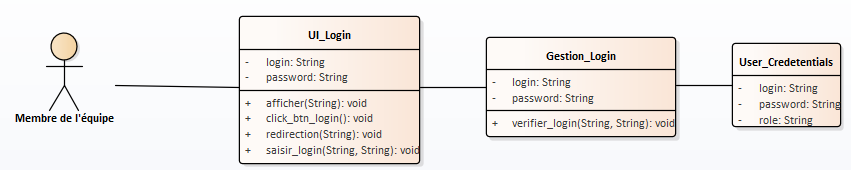
\includegraphics[scale=0.69]{figures/diagrams/class/authentification_class_diag.png}
 \caption{Diagramme de classes d'analyse de la fonctionnalité "s'authentifier"}
 \label{code60}
\end{figure}

\subsubsection{Ajouter un membre}
La figure \ref{code61} représente le diagramme de classes d'analyse de la fonctionnalité "ajouter un membre".
\begin{figure}[H]
  \centering
 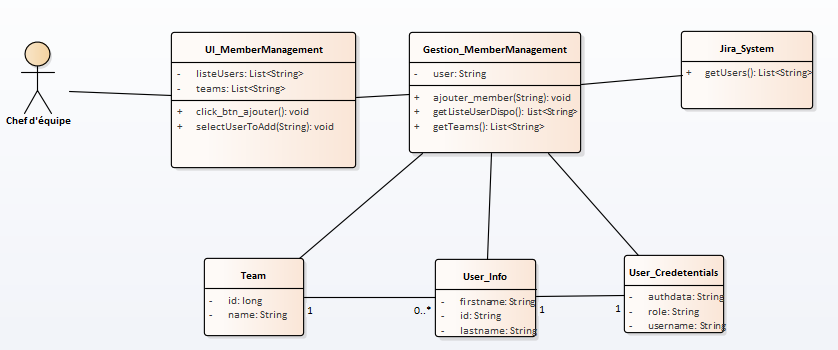
\includegraphics[scale=0.69]{figures/diagrams/class/addmember_class_diag.png}
 \caption{Diagramme de classes d'analyse de la fonctionnalité "Ajouter un membre"}
 \label{code61}
\end{figure}

\subsubsection{Consulter tout les tableaux de bord}
La figure \ref{code62} représente le diagramme de classes d'analyse de la fonctionnalité "Consulter tout les tableaux de bord".
\begin{figure}[H]
  \centering
 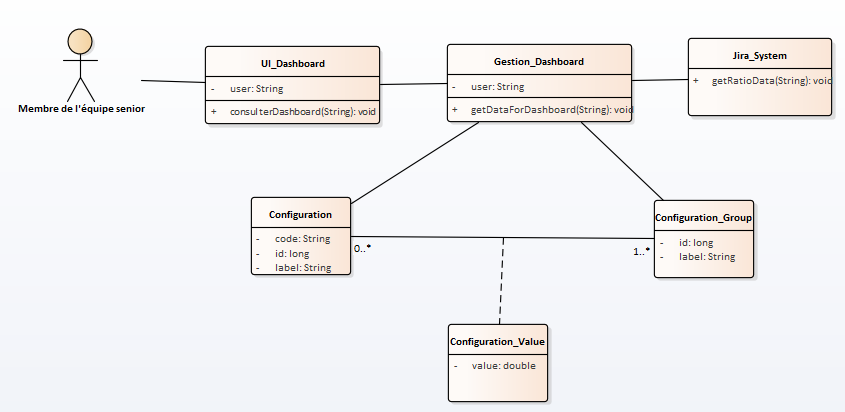
\includegraphics[scale=0.69]{figures/diagrams/class/consulteralldashboard_class_diag.png}
 \caption{Diagramme de classes d'analyse de la fonctionnalité "Consulter tout les tableaux de bord"}
 \label{code62}
\end{figure}

\newpage
\subsection{Modélisation dynamique}
%Diagramme de séquences détaillé ou état transition%
La modélisation dynamique permet d'avoir une idée sur le flux d'exécution de notre application. Nous présentons donc les diagrammes de séquences pour chaque fonctionnalité.

\subsubsection{S'authentifier}
Pour s'authentifier, le membre de l'équipe saisie son nom d'utilisateur et son mot de passe. Puis, il valide par le bouton login. Si la combinaison est incorrecte, un message d'erreur apparaît. Sinon, l'utilisateur est redirigé vers la page d'accueil.
La figure \ref{code57} représente le diagramme de séquence de la fonctionnalité "s'authentifier".
\begin{figure}[H]
  \centering
  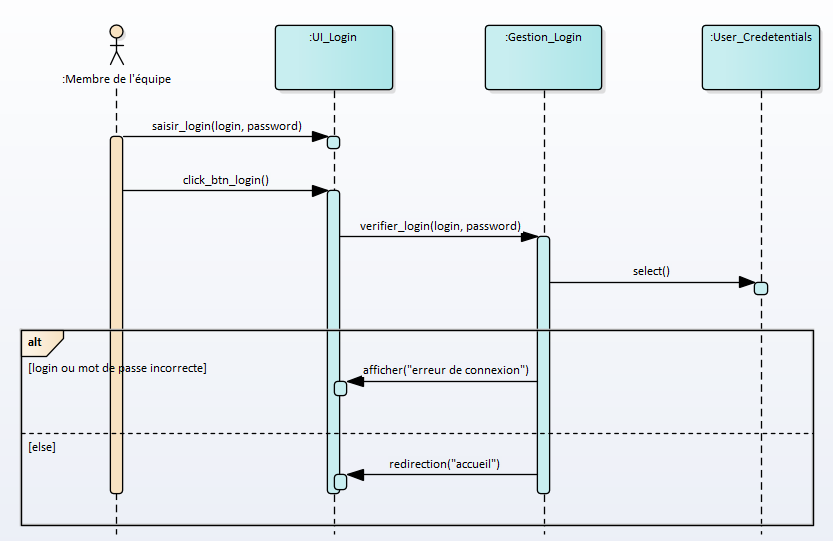
\includegraphics[scale=0.7]{figures/diagrams/sequence/authentification_seq_diag.png}
  \caption{Diagramme de séquence de la fonctionnalité "S'authentifier"}
  \label{code57}
\end{figure}

\subsubsection{Ajouter un membre}
Pour ajouter un membre, le chef d'équipe doit sélectionner le nom du membre à ajouter. Puis, il valide par le bouton ajouter.
La figure \ref{code58} représente le diagramme de séquence de la fonctionnalité "ajouter un membre".
\begin{figure}[H]
  \centering
 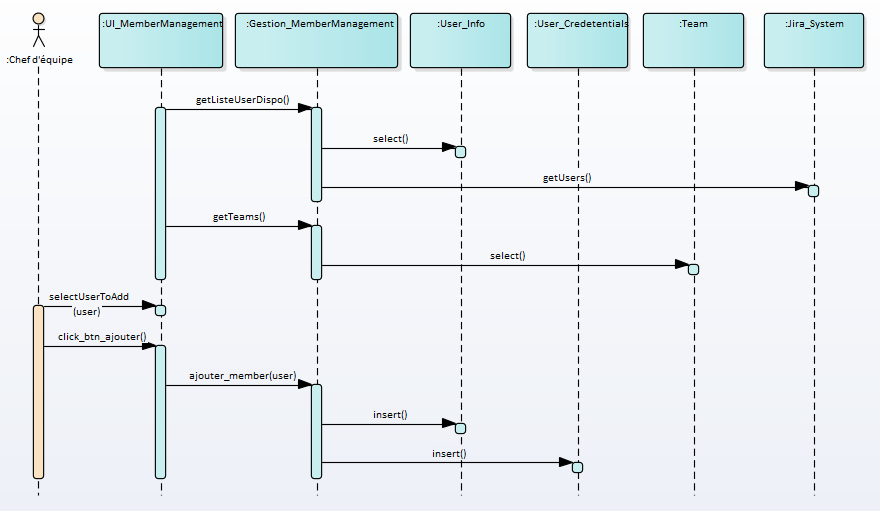
\includegraphics[scale=0.7]{figures/diagrams/sequence/ajoutermembre_seq_diag.png}
 \caption{Diagramme de séquence de la fonctionnalité "Ajouter un membre"}
 \label{code58}
\end{figure}

\subsubsection{Consulter tout les tableaux de bord}
Pour consulter tout les tableaux de bord, le membre de l'équipe senior doit cliquer sur le bouton consulter tableau de bord.
La figure \ref{code59} représente le diagramme de séquence de la fonctionnalité "consulter tout les tableaux de bord".
\begin{figure}[H]
  \centering
 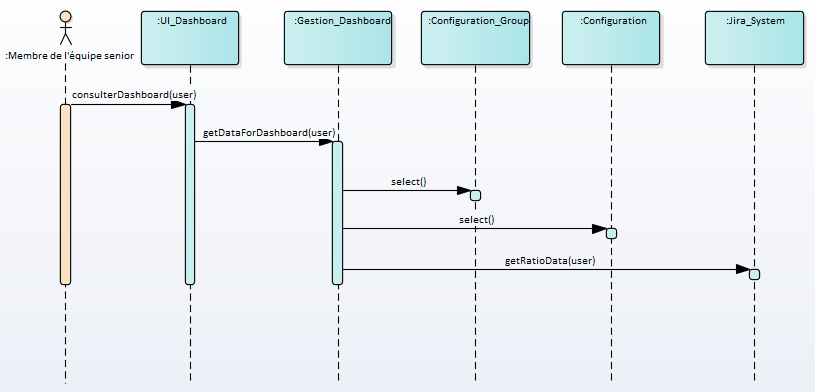
\includegraphics[scale=0.69]{figures/diagrams/sequence/consulteralldashboard_seq_diag.png}
 \caption{Diagramme de séquence de la fonctionnalité "Consulter tout les tableaux de bord"}
 \label{code59}
\end{figure}

\subsection{Développement du sprint}
%Capture d'écrans%
Le but de cette section est de montrer l'acheminement du sprint en présentant des captures d'écrans des fonctionnalités réalisés dans ce sprint.

\subsubsection{S'authentifier}
L'utilisateur saisit son nom d'utilisateur et son mot de passe. S'il se trompe dans l'un d'eux, un message d'erreur apparaît. Sinon l'écran d'accueil apparaît.
La figure \ref{code83} représente le message d'erreur reçu lorsqu'on se trompe de nom d'utilisateur ou de mot de passe.
\begin{figure}[H]
  \centering
 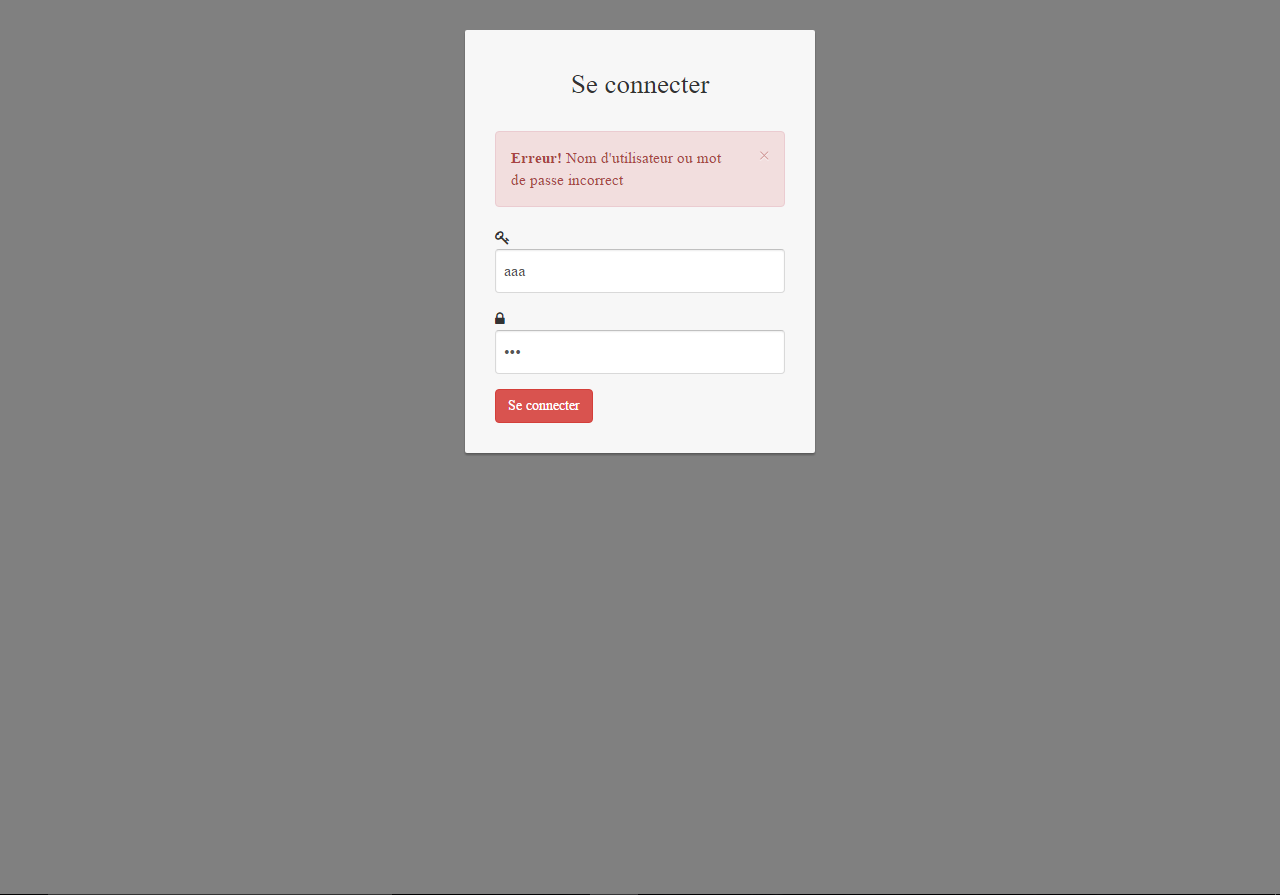
\includegraphics[scale=0.4]{figures/printscreen_app/1_1.PNG}
 \caption{Capture d'écran: mot de passe incorrecte}
 \label{code83}
\end{figure}
Si le mot de passe est correcte, l'utilisateur se retrouve à l'écran d'accueil.
\subsubsection{Ajouter un membre}
Les utilisateurs qui ont un compte jira mais qui n'ont pas un compte dans notre application sont automatiquement chargé dans la liste des utilisateurs à ajouter. On remplis les champs privilège et équipe puis on valide avec le bouton ajouter. Le message de validation d'ajout est représenté par la figure \ref{code84}.
\begin{figure}[H]
  \centering
 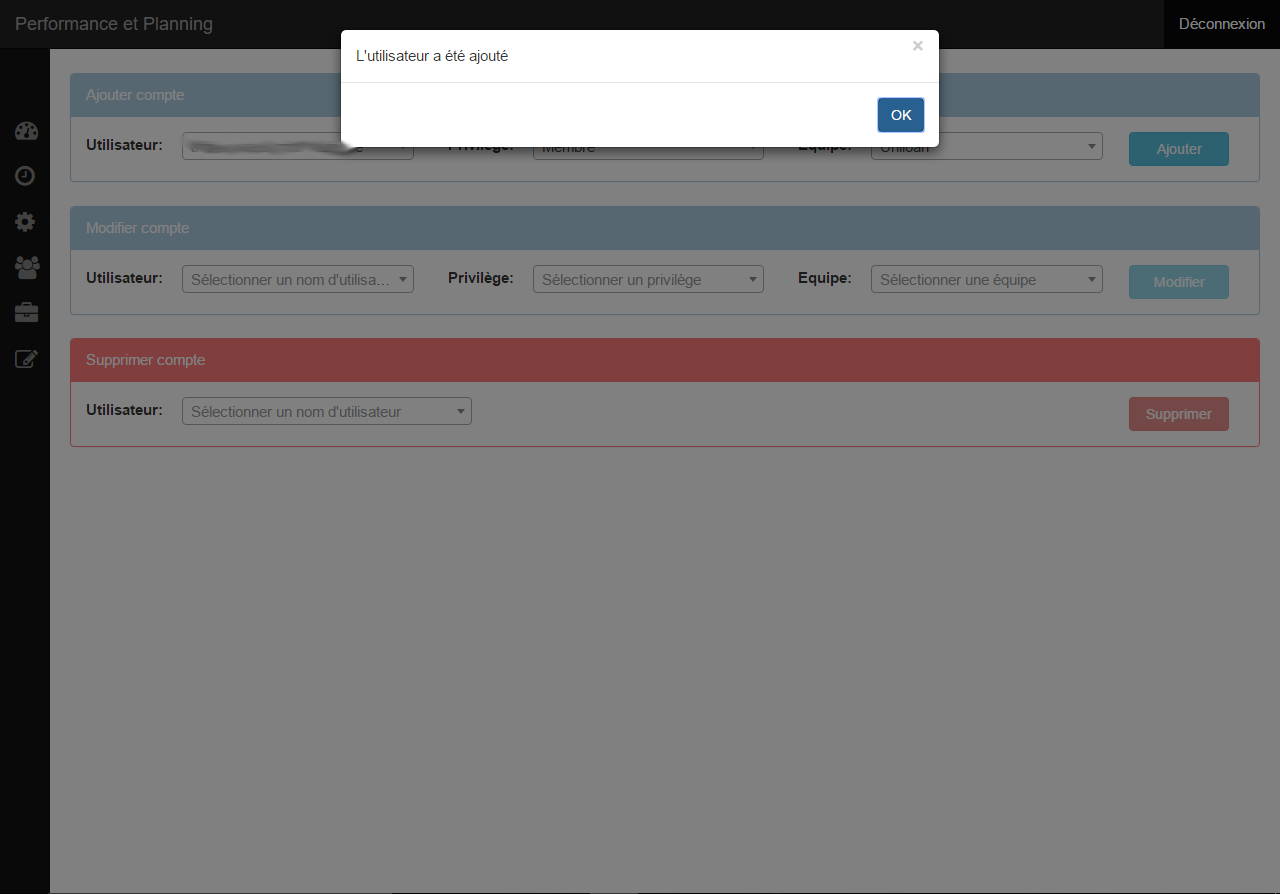
\includegraphics[scale=0.4]{figures/printscreen_app/2_2.PNG}
 \caption{Capture d'écran: ajouter membre}
 \label{code84}
\end{figure}
\subsubsection{Consulter tout les tableaux de bord}
Le membre de l'équipe senior ou le chef d'équipe peuvent consulter tout les tableaux de bord de leur équipe. Une partie du tableau de bord d'un membre de l'équipe est représenté dans la figure \ref{code85}.
\begin{figure}[H]
  \centering
 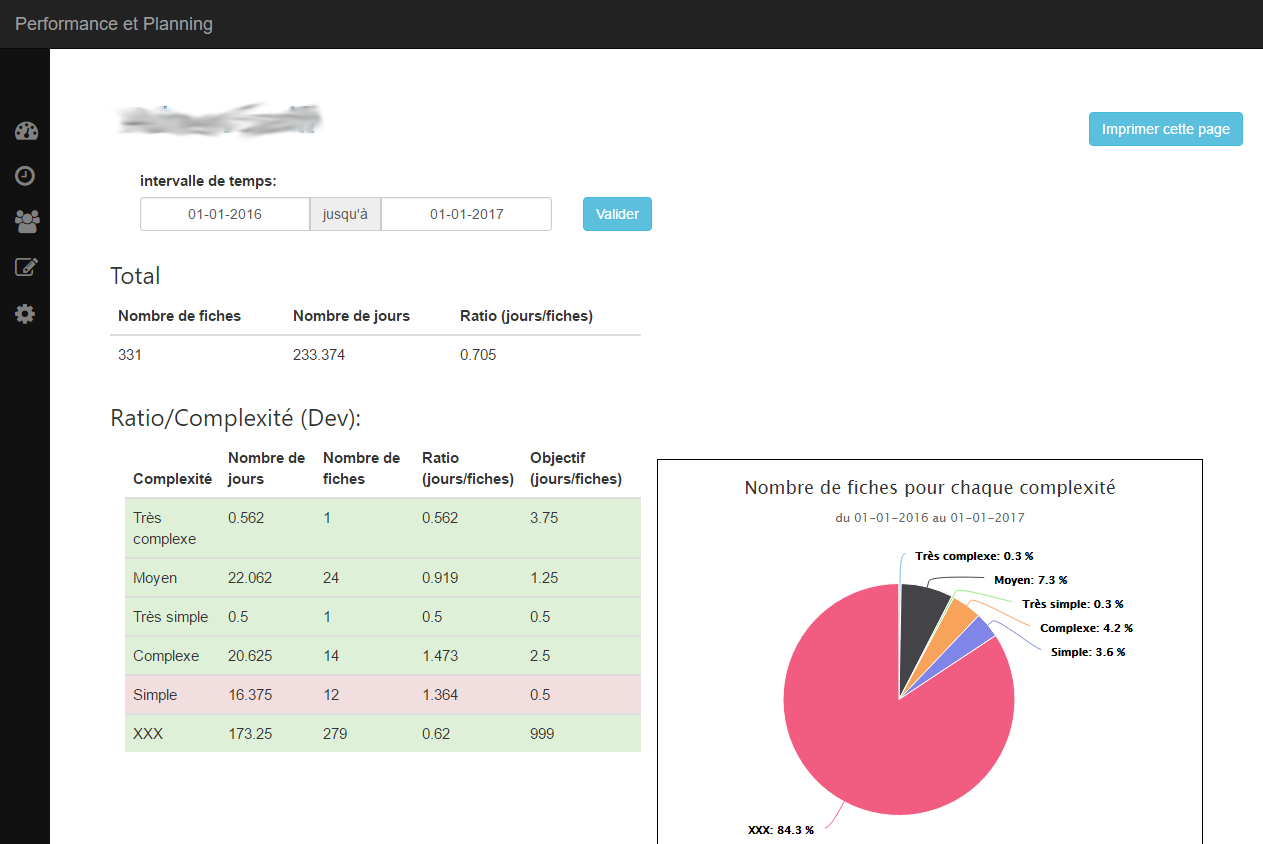
\includegraphics[scale=0.35]{figures/printscreen_app/3_1.PNG}
 \caption{Capture d'écran: partie d'un tableau de bord d'un membre}
 \label{code85}
\end{figure}

\subsection{Test et revue du sprint}
%Burndown chart%
Dans cette section, nous allons présenté l'avancement de notre sprint sous forme de burndown chart. La figure \ref{code86} représente la burndown chart de notre sprint.
\begin{figure}[H]
  \centering
 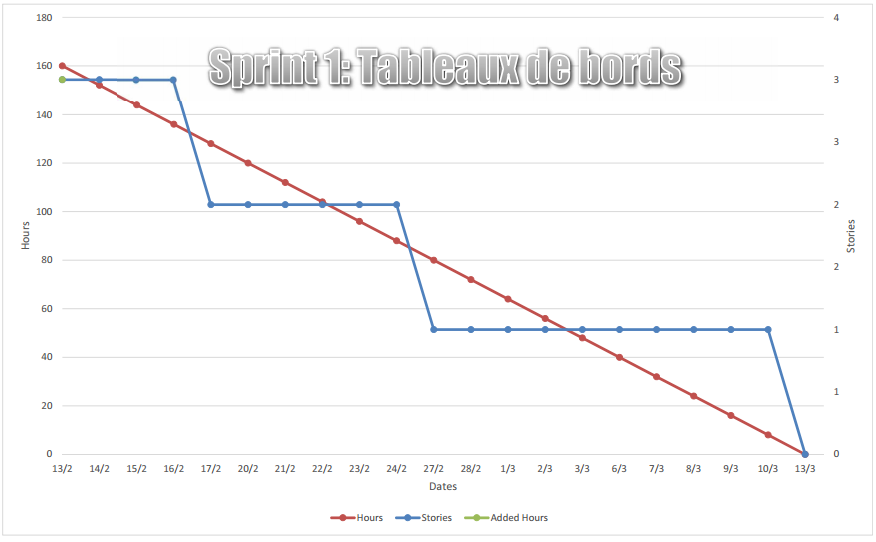
\includegraphics[scale=0.7]{figures/burndown_chart/sprint1.png}
 \caption{Burndown Chart du sprint 1: Tableaux de bord}
 \label{code86}
\end{figure}

\subsection{Rétrospective}
Cette section est dédiée à l'énumération des problèmes rencontrés dans ce sprint. Ces derniers se résument comme suit:
\begin{itemize}
    \item[$\bullet$] Se familiariser avec la base de données Jira qui contient trop de tables sans clés étrangères.
    \item[$\bullet$] Se familiariser avec les techniques de cryptage et hashage pour pouvoir sécuriser l'authentification.
    \item[$\bullet$] Comprendre les différents indicateurs de performances pour pouvoir créer les tableaux de bord.
\end{itemize}

\section{Sprint 2: Tableau de bord de l'équipe (du 13-03-2017 au 10-04-2017)}
Dans cette section, nous allons détailler la réalisation du sprint 2. En premier lieu, nous allons présenter la planification du sprint en présentant le but du sprint et le backlog sprint. Ensuite nous allons spécifier la modélisation statique et la modélisation dynamique. Puis, nous allons présenter le développement du sprint sous forme de capture d'écrans. Et nous finirons, enfin, avec le test, la revue et la rétrospective du sprint.

\subsection{Sprint planning}
%But du sprint + backlog sprint%
Le but de ce sprint est de créer des tableaux de bords de l'équipe fonctionnels qui utilisent des données de notre base de données Jira. De ce fait, nous proposons le backlog sprint qui est représenté dans la table \ref{code63}.
\begin{longtable}{l}
\caption{Backlog du sprint2: "Tableau de bord de l'équipe"} \label{code63} \\
\begin{tabular}{|c|l|l|l|}
\hline
\multicolumn{1}{|l|}{\textbf{User storyID}} & \textbf{User Story} & \textbf{Tâche ID} & \textbf{Tâche} \\ \hline
\multirow{3}{*}{2.1} & \multirow{3}{*}{\begin{tabular}[c]{@{}l@{}}En tant que chef d’équipe, \\ je souhaite\\ pouvoir créer \\ une nouvelle équipe.\end{tabular}} & 2.1.1 & \begin{tabular}[c]{@{}l@{}}Réaliser les diagrammes UML \\ de la fonctionnalité "créer une \\ équipe".\end{tabular} \\ \cline{3-4} 
 &  & 2.1.2 & \begin{tabular}[c]{@{}l@{}}Développer la fonctionnalité \\ "créer une équipe".\end{tabular} \\ \cline{3-4} 
 &  & 2.1.3 & \begin{tabular}[c]{@{}l@{}}Tester la fonctionnalité \\ "créer une équipe".\end{tabular} \\ \hline
\multirow{3}{*}{2.2} & \multirow{3}{*}{\begin{tabular}[c]{@{}l@{}}En tant que chef d’équipe, \\ je souhaite\\ pouvoir \\ supprimer une équipe.\end{tabular}} & 2.2.1 & \begin{tabular}[c]{@{}l@{}}Réaliser les diagrammes UML \\ de la fonctionnalité "supprimer \\ une équipe".\end{tabular} \\ \cline{3-4} 
 &  & 2.2.2 & \begin{tabular}[c]{@{}l@{}}Développer la fonctionnalité \\ "supprimer une équipe".\end{tabular} \\ \cline{3-4} 
 &  & 2.2.3 & \begin{tabular}[c]{@{}l@{}}Tester la fonctionnalité \\ "supprimer une équipe".\end{tabular} \\ \hline
\multirow{3}{*}{3.2} & \multirow{3}{*}{\begin{tabular}[c]{@{}l@{}}En tant que chef d’équipe, \\ je souhaite\\ pouvoir \\ supprimer un membre de\\ \\ l’application.\end{tabular}} & 3.2.1 & \begin{tabular}[c]{@{}l@{}}Réaliser les diagrammes UML\\  de la fonctionnalité \\ "supprimer un membre".\end{tabular} \\ \cline{3-4} 
 &  & 3.2.2 & \begin{tabular}[c]{@{}l@{}}Développer la fonctionnalité \\ "supprimer un membre".\end{tabular} \\ \cline{3-4} 
 &  & 3.2.3 & \begin{tabular}[c]{@{}l@{}}Tester la fonctionnalité \\ "supprimer un membre".\end{tabular} \\ \hline
\multirow{3}{*}{3.3} & \multirow{3}{*}{\begin{tabular}[c]{@{}l@{}}En tant que chef d’équipe, \\ je souhaitepouvoir modifier \\ un membre de\\ l’application.\end{tabular}} & 3.3.1 & \begin{tabular}[c]{@{}l@{}}Réaliser les diagrammes UML \\ de la fonctionnalité "modifier \\ un membre".\end{tabular} \\ \cline{3-4} 
 &  & 3.3.2 & \begin{tabular}[c]{@{}l@{}}Développer la fonctionnalité \\ "modifier un membre".\end{tabular} \\ \cline{3-4} 
 &  & 3.3.3 & \begin{tabular}[c]{@{}l@{}}Tester la fonctionnalité \\ "modifier un membre".\end{tabular} \\ \hline
\end{tabular} \\
\begin{tabular}{|c|l|l|l|}
\hline
\multicolumn{1}{|l|}{\textbf{User storyID}} & \textbf{User Story} & \textbf{Tâche ID} & \textbf{Tâche} \\ \hline
\multirow{3}{*}{4.1} & \multirow{3}{*}{\begin{tabular}[c]{@{}l@{}}En tant que membre senior \\ ou chef\\ d’équipe, je souhaite \\ pouvoir consulter\\ le tableaux \\ de bord de l’équipe.\end{tabular}} & 4.1.1 & \begin{tabular}[c]{@{}l@{}}Réaliser les diagrammes UML \\ de la fonctionnalité "consulter \\ le tableau de bord de l'équipe".\end{tabular} \\ \cline{3-4} 
 &  & 4.1.2 & \begin{tabular}[c]{@{}l@{}}Développer la fonctionnalité \\ "consulter le tableau de bord \\ de l'équipe".\end{tabular} \\ \cline{3-4} 
 &  & 4.1.3 & \begin{tabular}[c]{@{}l@{}}Tester la fonctionnalité \\ "consulter le tableau de \\ bord de l'équipe".\end{tabular} \\ \hline
\multirow{3}{*}{6.1} & \multirow{3}{*}{\begin{tabular}[c]{@{}l@{}}En tant que chef d’équipe, \\ je souhaite pouvoir \\ modifier les valeurs des\\ objectifs ICP.\end{tabular}} & 6.1.1 & \begin{tabular}[c]{@{}l@{}}Réaliser les diagrammes UML \\ de la fonctionnalité "modifier \\ les valeurs des objectifs ICP".\end{tabular} \\ \cline{3-4} 
 &  & 6.1.2 & \begin{tabular}[c]{@{}l@{}}Développer la fonctionnalité \\ "modifier les valeurs des \\ objectifs ICP".\end{tabular} \\ \cline{3-4} 
 &  & 6.1.3 & \begin{tabular}[c]{@{}l@{}}Tester la fonctionnalité \\ "modifier les valeurs des \\ objectifs ICP".\end{tabular} \\ \hline
\end{tabular}
\end{longtable}

\subsection{Modélisation statique}
%Diagramme de classes%
Nous présentons dans cette partie la modélisation statique de ce sprint sous forme de diagrammes de classes d'analyse pour chaque fonctionnalité.

\subsubsection{Créer une équipe}
La figure \ref{code64} représente le diagramme de classes d'analyse de la fonctionnalité "créer une équipe".
\begin{figure}[H]
  \centering
 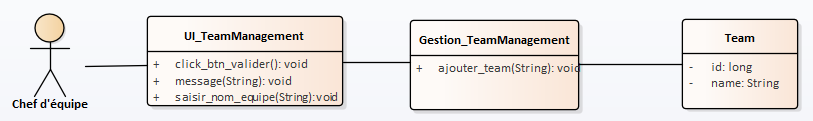
\includegraphics[scale=0.69]{figures/diagrams/class/createteam_class_diag.png}
 \caption{Diagramme de classes d'analyse de la fonctionnalité "créer une équipe"}
 \label{code64}
\end{figure}

\subsubsection{Supprimer une équipe}
La figure \ref{code65} représente le diagramme de classes d'analyse de la fonctionnalité "supprimer une équipe".
\begin{figure}[H]
  \centering
 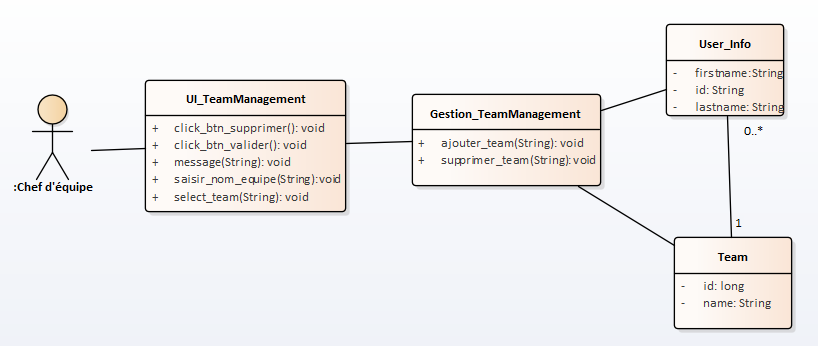
\includegraphics[scale=0.69]{figures/diagrams/class/deleteteam_class_diag.png}
 \caption{Diagramme de classes d'analyse de la fonctionnalité "supprimer une équipe"}
 \label{code65}
\end{figure}

\subsubsection{Modifier un membre}
La figure \ref{code66} représente le diagramme de classes d'analyse de la fonctionnalité "modifier un membre".
\begin{figure}[H]
  \centering
 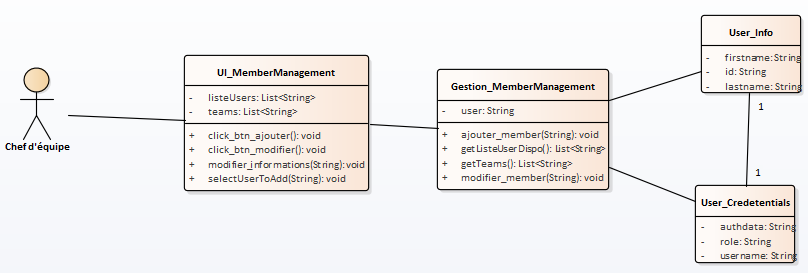
\includegraphics[scale=0.69]{figures/diagrams/class/updatemember_class_diag.png}
 \caption{Diagramme de classes d'analyse de la fonctionnalité "modifier un membre"}
 \label{code66}
\end{figure}

\subsubsection{Supprimer un membre}
La figure \ref{code67} représente le diagramme de classes d'analyse de la fonctionnalité "supprimer un membre".
\begin{figure}[H]
  \centering
 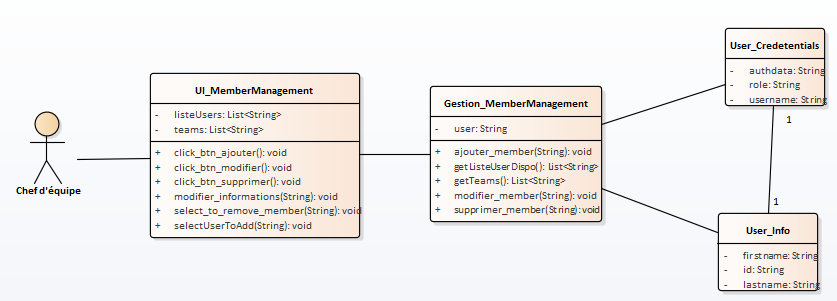
\includegraphics[scale=0.69]{figures/diagrams/class/deletemember_class_diag.png}
 \caption{Diagramme de classes d'analyse de la fonctionnalité "supprimer un membre"}
 \label{code67}
\end{figure}

\subsubsection{Consulter le tableau de bord de l'équipe}
La figure \ref{code68} représente le diagramme de classes d'analyse de la fonctionnalité "consulter le tableau de bord de l'équipe".
\begin{figure}[H]
  \centering
 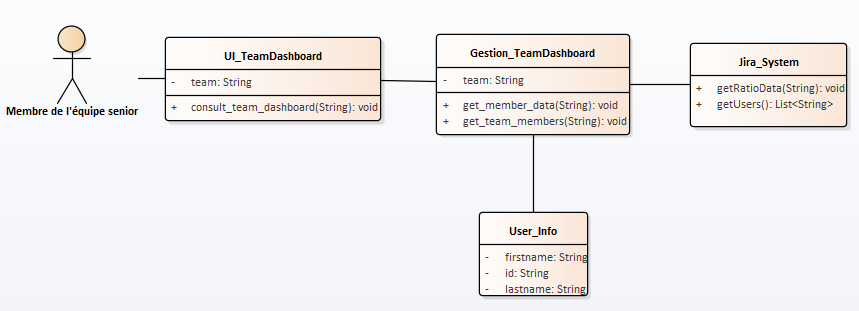
\includegraphics[scale=0.69]{figures/diagrams/class/teamdashboard_class_diag.png}
 \caption{Diagramme de classes d'analyse de la fonctionnalité "consulter le tableau de bord de l'équipe"}
 \label{code68}
\end{figure}

\subsubsection{Modifier les valeurs des objectifs ICP}
La figure \ref{code69} représente le diagramme de classes d'analyse de la fonctionnalité "modifier les valeurs des objectifs ICP".
\begin{figure}[H]
  \centering
 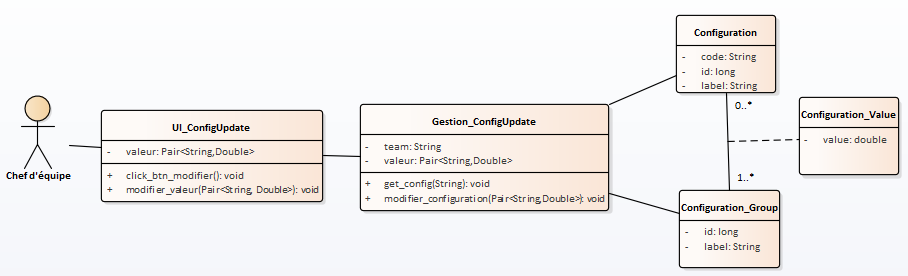
\includegraphics[scale=0.69]{figures/diagrams/class/config_class_diag.png}
 \caption{Diagramme de classes d'analyse de la fonctionnalité "modifier les valeurs des objectifs ICP"}
 \label{code69}
\end{figure}

\subsection{Modélisation dynamique}
%Diagramme de séquences détaillé ou état transition%
Nous présentons dans cette partie la modélisation dynamique de ce sprint sous forme de diagrammes de séquences pour chaque fonctionnalité.

\subsubsection{Créer une équipe}
Pour créer une équipe, le chef d'équipe saisie le nom d'une équipe à ajouter. Puis, il clique sur le bouton valider. Si le nom n'existe pas dans la base de données, l'équipe est automatiquement ajoutée et un message validant l'ajout apparaît. Sinon, un message d'erreur apparaît sur l'écran.
La figure \ref{code70} représente le diagramme de séquence de la fonctionnalité "créer une équipe".
\begin{figure}[H]
  \centering
 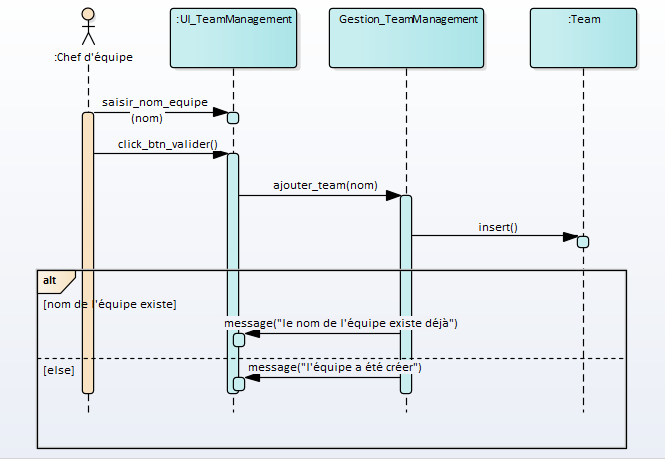
\includegraphics[scale=0.69]{figures/diagrams/sequence/createteam_seq_diag.png}
 \caption{Diagramme de séquence de la fonctionnalité "créer une équipe"}
 \label{code70}
\end{figure}

\subsubsection{Supprimer une équipe}
Pour supprimer une équipe, le chef d'équipe sélectionne le nom de l'équipe à supprimer. Puis, il valide par le bouton valider. l'équipe est alors supprimée.
La figure \ref{code71} représente le diagramme de séquence de la fonctionnalité "supprimer une équipe".
\begin{figure}[H]
  \centering
 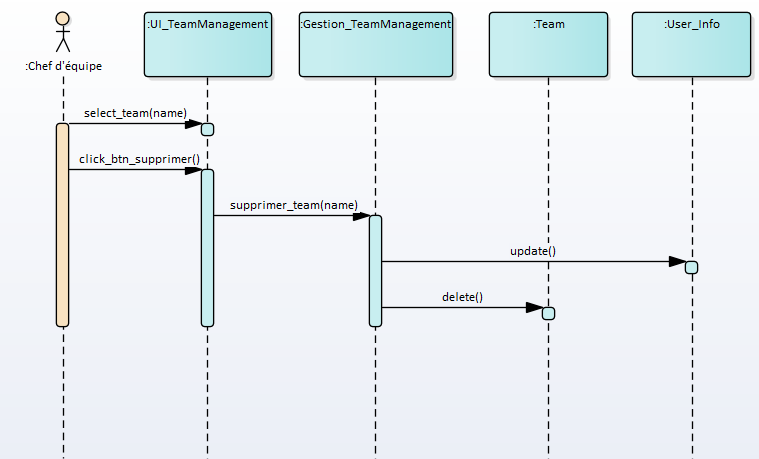
\includegraphics[scale=0.69]{figures/diagrams/sequence/deleteteam_seq_diag.png}
 \caption{Diagramme de séquence de la fonctionnalité "supprimer une équipe"}
 \label{code71}
\end{figure}

\subsubsection{Modifier un membre}
Pour modifier un membre, le chef d'équipe sélectionne le nom du membre à modifier. Puis, il fait les changements nécessaires et il valide par le bouton valider.
La figure \ref{code72} représente le diagramme de séquence de la fonctionnalité "modifier un membre".
\begin{figure}[H]
  \centering
 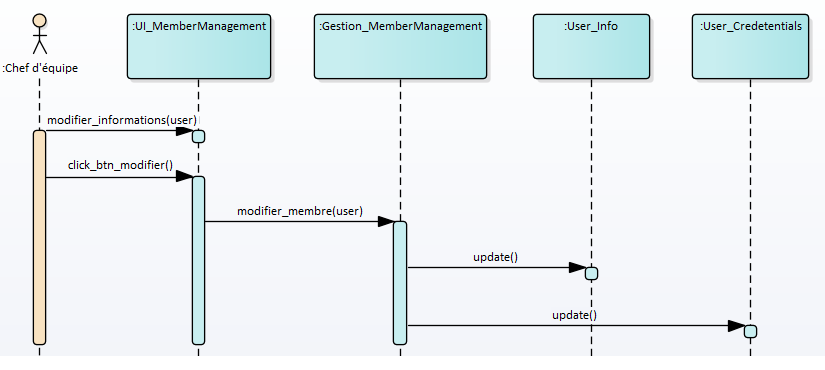
\includegraphics[scale=0.65]{figures/diagrams/sequence/updatemember_seq_diag.png}
 \caption{Diagramme de séquence de la fonctionnalité "modifier un membre"}
 \label{code72}
\end{figure}

\subsubsection{Supprimer un membre}
Pour supprimer un membre, le chef d'équipe sélectionne le nom du membre à supprimer. Puis, il valide par le bouton supprimer.
La figure \ref{code73} représente le diagramme de séquence de la fonctionnalité "supprimer un membre".
\begin{figure}[H]
  \centering
 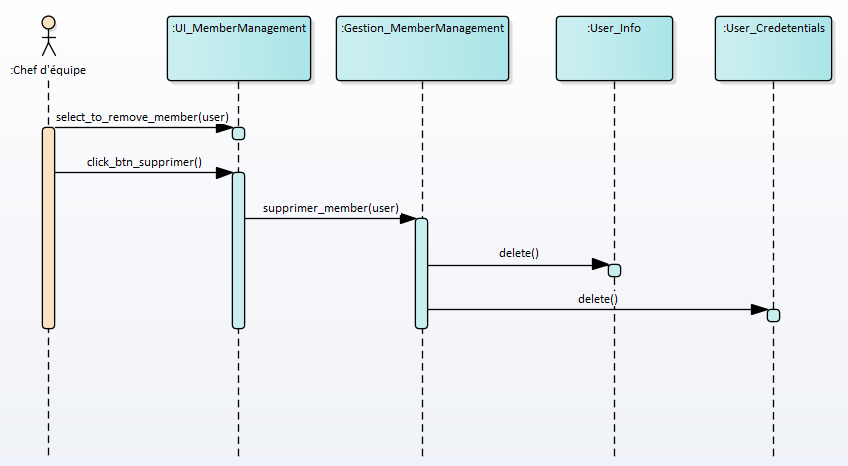
\includegraphics[scale=0.69]{figures/diagrams/sequence/deletemember_seq_diag.png}
 \caption{Diagramme de séquence de la fonctionnalité "supprimer un membre"}
 \label{code73}
\end{figure}

\subsubsection{Consulter le tableau de bord de l'équipe}
Pour consulter le tableau de bord de l'équipe, le membre de l'équipe senior clique sur le bouton consulter.
La figure \ref{code74} représente le diagramme de séquence de la fonctionnalité "consulter le tableau de bord de l'équipe".
\begin{figure}[H]
  \centering
 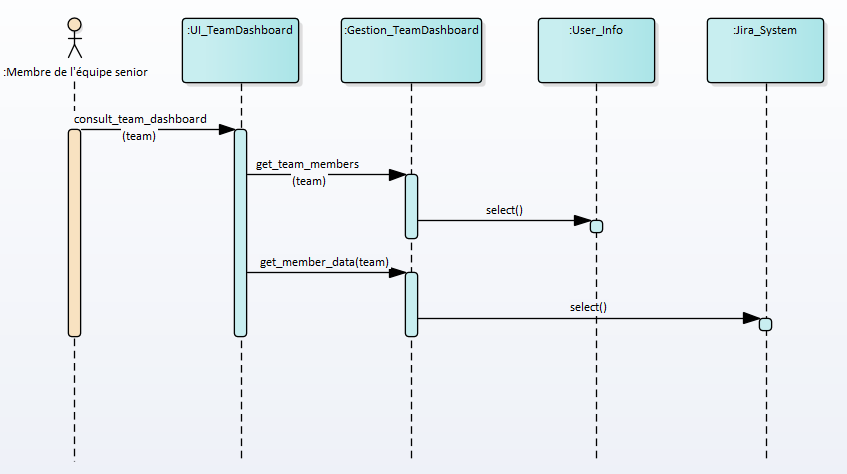
\includegraphics[scale=0.69]{figures/diagrams/sequence/teamdashboard_seq_diag.png}
 \caption{Diagramme de séquence de la fonctionnalité "consulter le tableau de bord de l'équipe"}
 \label{code74}
\end{figure}

\subsubsection{Modifier les valeurs des objectifs ICP}
Pour modifier les valeurs des objectifs ICP, le chef d'équipe modifie les valeurs des champs dans la page. Puis, il valide par le bouton modifier.
La figure \ref{code75} représente le diagramme de séquence de la fonctionnalité "modifier les valeurs des objectifs ICP".
\begin{figure}[H]
  \centering
 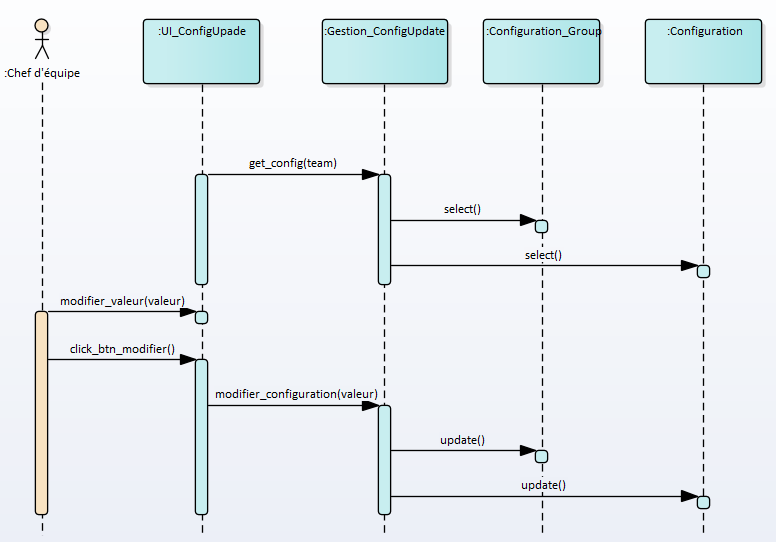
\includegraphics[scale=0.69]{figures/diagrams/sequence/config_seq_diag.png}
 \caption{Diagramme de séquence de la fonctionnalité "modifier les valeurs des objectifs ICP"}
 \label{code75}
\end{figure}

\subsection{Développement du sprint}
%Capture d'écrans%
Le but de cette section est de montrer l'acheminement du sprint en présentant des captures d'écrans des fonctionnalités réalisés dans ce sprint.

\subsubsection{Créer une équipe}
L'utilisateur saisit le nom de l'équipe qu'il veut ajouter. Si le nom existe dans la base de données, un message d'avertissement apparaît et le bouton d'ajout se désactive. Sinon l'équipe est ajoutée dans la base de données. La figure \ref{code87} représente le message de validation d'ajout d'une équipe.
\begin{figure}[H]
  \centering
 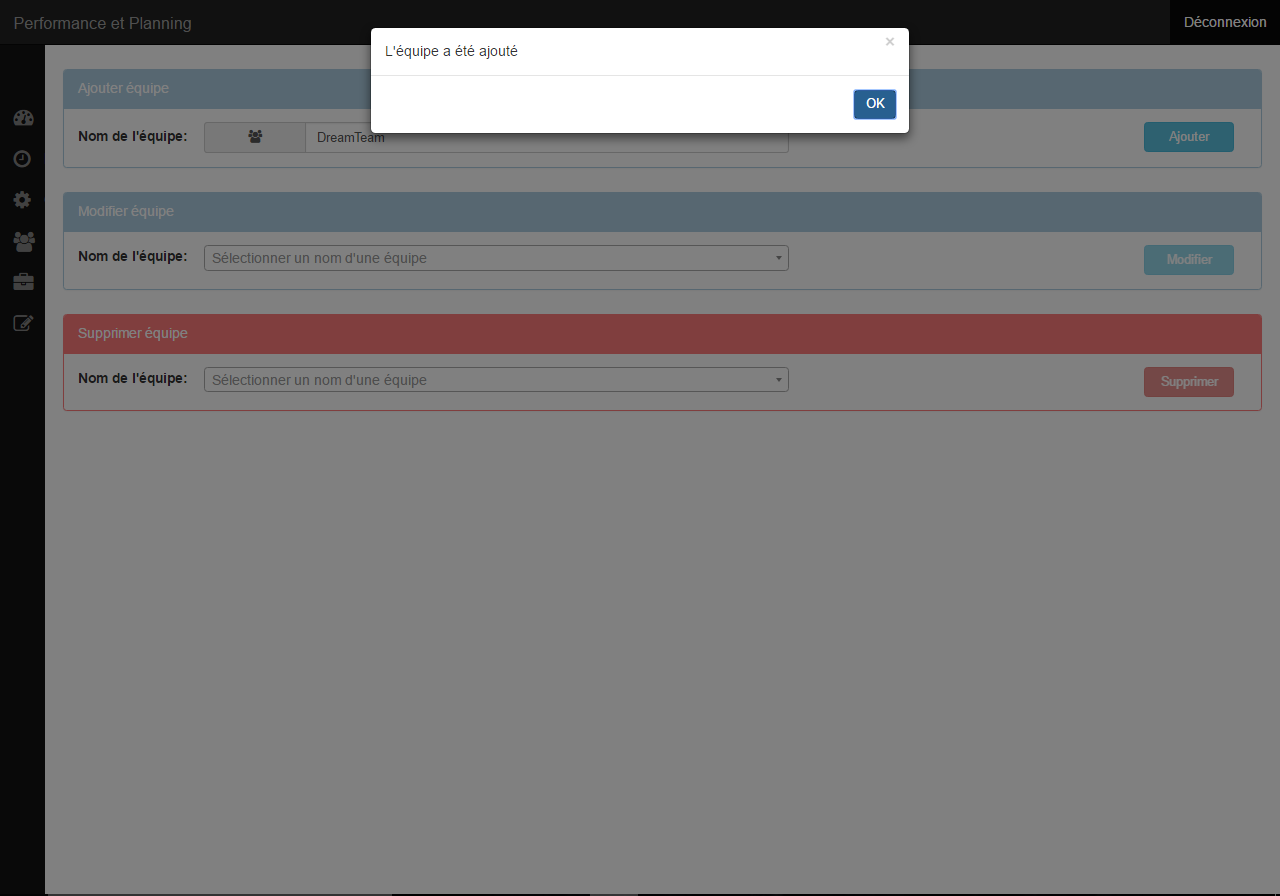
\includegraphics[scale=0.37]{figures/printscreen_app/4_2.PNG}
 \caption{Capture d'écran: créer une équipe}
 \label{code87}
\end{figure}

\subsubsection{Supprimer une équipe}
L'utilisateur sélectionne l'équipe à supprimer puis il clique sur le bouton supprimer. L'équipe est alors supprimée de la base de données. La figure \ref{code88} représente le message de validation de suppression d'une équipe.
\begin{figure}[H]
  \centering
 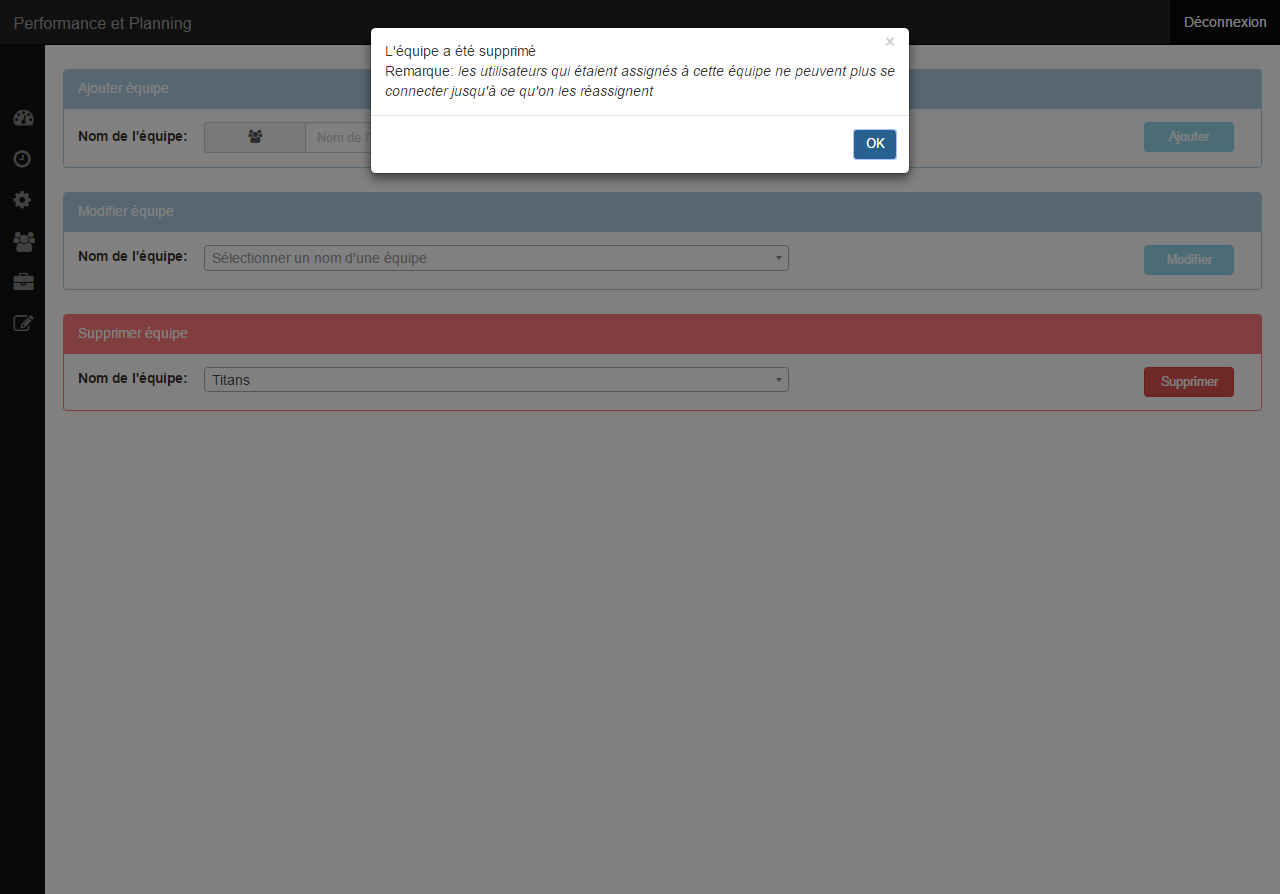
\includegraphics[scale=0.37]{figures/printscreen_app/5_3.PNG}
 \caption{Capture d'écran: supprimer une équipe}
 \label{code88}
\end{figure}

\subsubsection{Modifier un membre}
L'utilisateur sélectionne le membre à modifier. Puis il fait les changements nécessaires et il valide par le bouton modifier. La figure \ref{code89} représente le message de validation de modification d'un membre.
\begin{figure}[H]
  \centering
 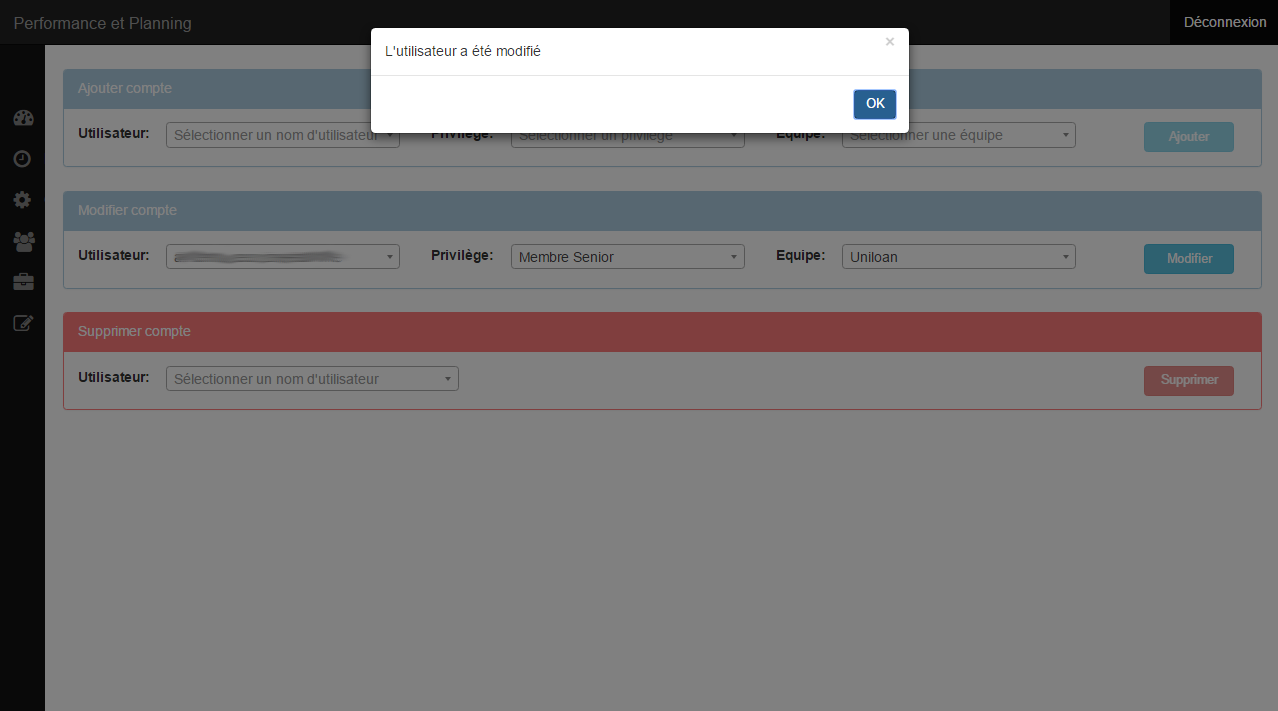
\includegraphics[scale=0.37]{figures/printscreen_app/6_3.PNG}
 \caption{Capture d'écran: modifier un membre}
 \label{code89}
\end{figure}

\subsubsection{Supprimer un membre}
L'utilisateur sélectionne le membrer à supprimer puis il clique sur le bouton supprimer. Le membre est alors supprimée de la base de données. La figure \ref{code90} représente le message de validation de suppression d'un membre.
\begin{figure}[H]
  \centering
 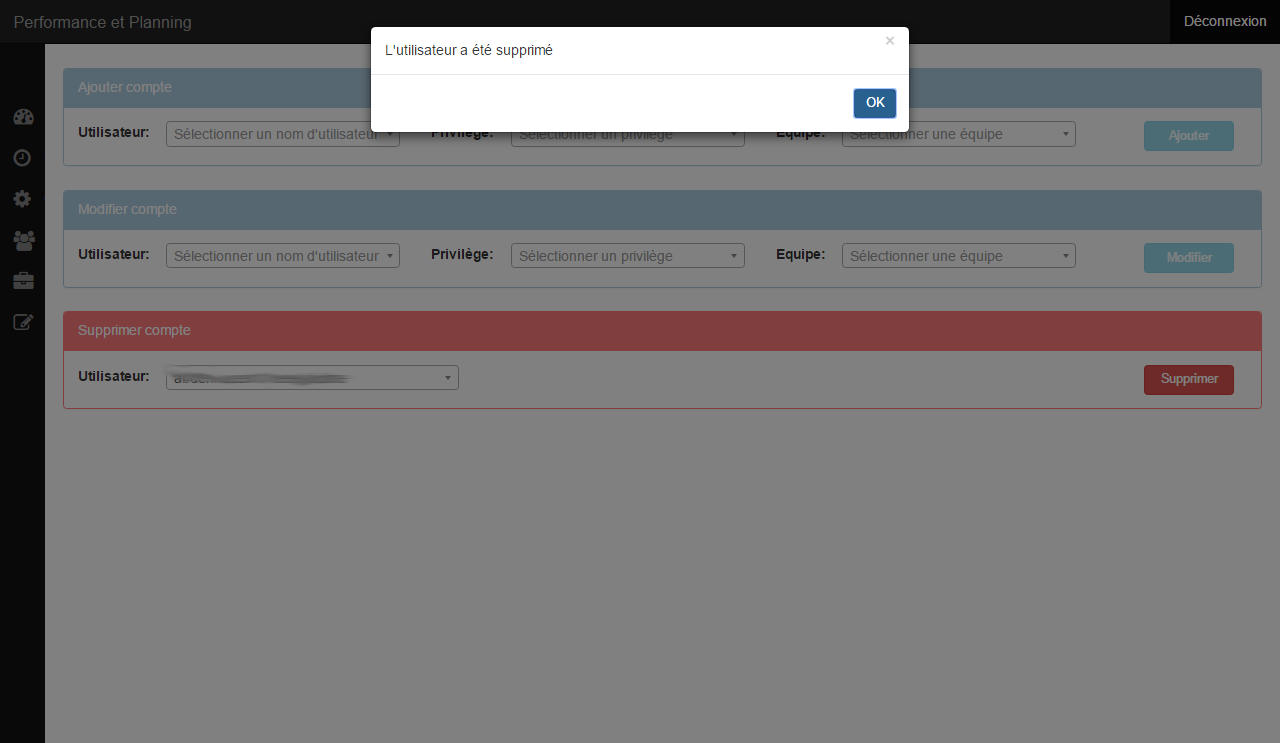
\includegraphics[scale=0.37]{figures/printscreen_app/7_3.PNG}
 \caption{Capture d'écran: supprimer un membre}
 \label{code90}
\end{figure}

\subsubsection{Consulter le tableau de bord de l'équipe}
L'utilisateur peut accéder au tableau de bord de l'équipe s'il clique sur le bouton "Tableau de bord" du menu vertical à gauche. La figure \ref{code91} représente le tableau de bord de l'équipe.
\begin{figure}[H]
  \centering
 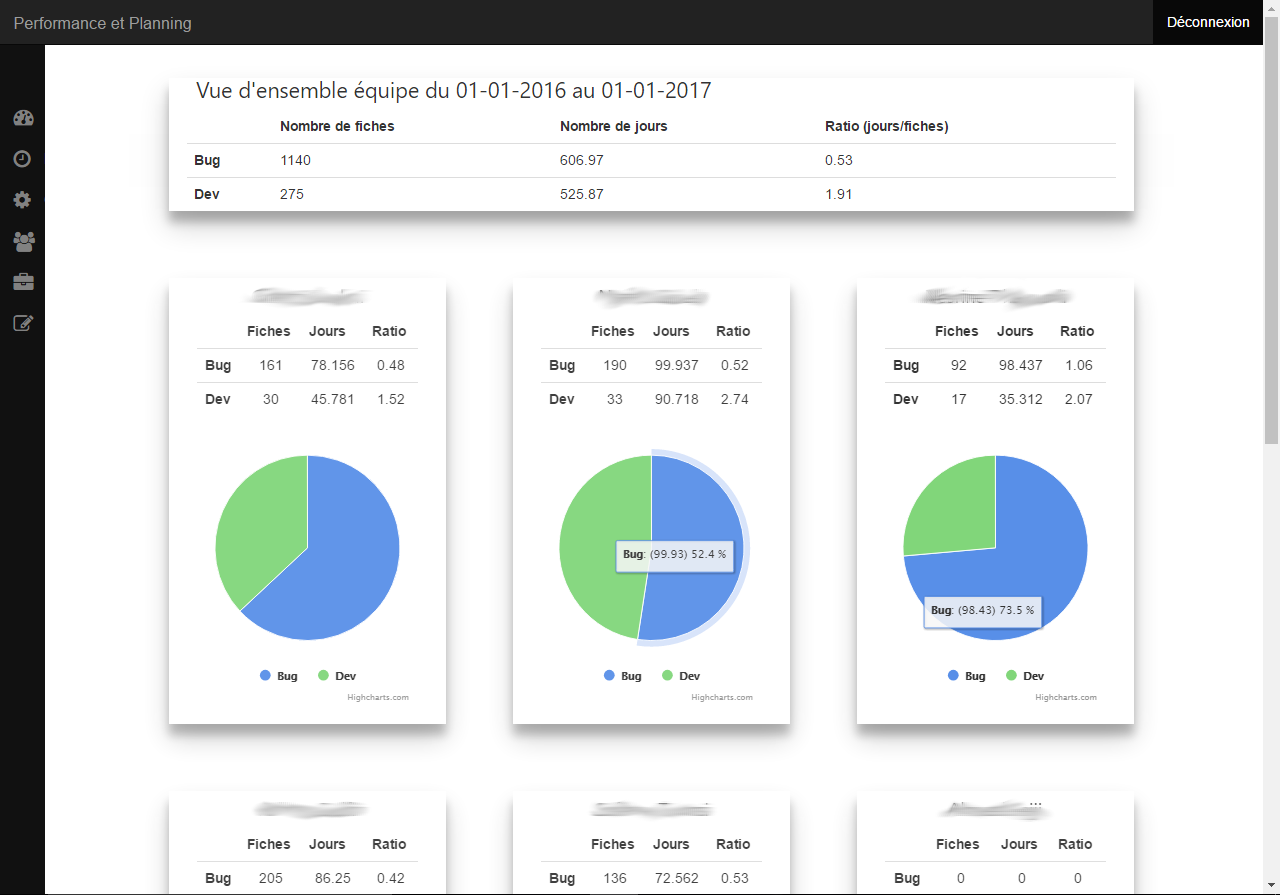
\includegraphics[scale=0.37]{figures/printscreen_app/8_2.PNG}
 \caption{Capture d'écran: tableau de bord de l'équipe}
 \label{code91}
\end{figure}

\subsubsection{Modifier les valeurs des objectifs ICP}
L'utilisateur peut modifier les valeurs des objectifs ICP puis il valide la modification en cliquant sur le bouton "Enregistrer les modifications". La figure \ref{code92} représente le message de validation des modifications.
\begin{figure}[H]
  \centering
 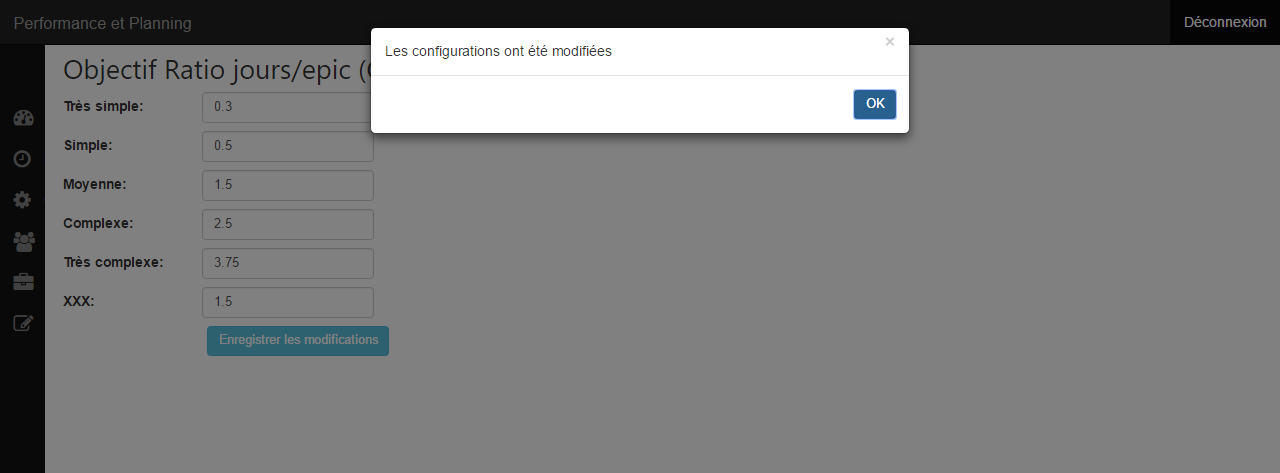
\includegraphics[scale=0.37]{figures/printscreen_app/9_3.PNG}
 \caption{Capture d'écran: tableau de bord de l'équipe}
 \label{code92}
\end{figure}

\subsection{Test et revue du sprint}
%Burndown chart%
Dans cette section, nous allons présenté l’avancement de notre sprint sous forme de burndown chart. La figure \ref{code93} représente la burndown chart de notre sprint.
\begin{figure}[H]
  \centering
 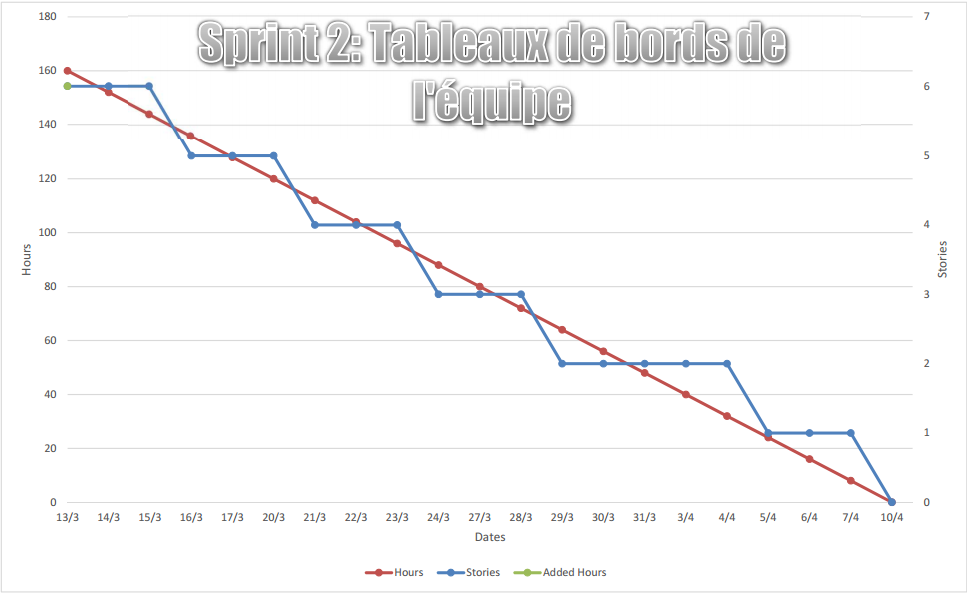
\includegraphics[scale=0.7]{figures/burndown_chart/sprint2.png}
 \caption{Burndown Chart du sprint 2: Tableaux de bord de l'équipe}
 \label{code93}
\end{figure}

\subsection{Rétrospective}
Cette section est dédiée à l'énumération des problèmes rencontrés dans ce sprint. Ces derniers se résument comme suit:
\begin{itemize}
    \item[$\bullet$] Pouvoir gérer les privilèges de chaque utilisateur de notre application
    \item[$\bullet$] Trouver une disposition relativement ergonomique pour afficher la liste de tout les membres de l'équipe.
\end{itemize}

\section{Sprint 3: Planification (du 10-04-2017 au 08-05-2017)}
Dans cette section, nous allons détailler la réalisation du sprint 3. En premier lieu, nous allons présenter la planification du sprint en présentant le but du sprint et le backlog sprint. Ensuite nous allons spécifier la modélisation statique et la modélisation dynamique. Puis, nous allons présenter le développement du sprint sous forme de capture d'écrans. Et nous finirons, enfin, avec le test, la revue et la rétrospective du sprint.

\subsection{Sprint planning}
%But du sprint + backlog sprint%
Le but de ce sprint est de créer des tableaux de bords de l'équipe fonctionnels qui utilisent des données de notre base de données Jira. De ce fait, nous proposons le backlog sprint qui est représenté dans la table \ref{code76}.
\begin{longtable}{l}
\caption{Backlog du sprint3: "Planification"} \label{code76} \\
\begin{tabular}{|c|l|l|l|}
\hline
\multicolumn{1}{|l|}{\textbf{User storyID}} & \textbf{User Story} & \textbf{Tâche ID} & \textbf{Tâche} \\ \hline
\multirow{3}{*}{1.2} & \multirow{3}{*}{\begin{tabular}[c]{@{}l@{}}En tant que membre, \\ membre senior ou chef \\ d’équipe, je souhaite \\ pouvoir modifier mon \\ mot de passe.\end{tabular}} & 2.1.1 & \begin{tabular}[c]{@{}l@{}}Réaliser les diagrammes UML \\ de la fonctionnalité "modifier \\ le mot de passe".\end{tabular} \\ \cline{3-4} 
 &  & 2.1.2 & \begin{tabular}[c]{@{}l@{}}Développer la fonctionnalité \\ "modifier le mot de passe".\end{tabular} \\ \cline{3-4} 
 &  & 2.1.3 & \begin{tabular}[c]{@{}l@{}}Tester la fonctionnalité \\ "modifier le mot de passe".\end{tabular} \\ \hline
\multirow{3}{*}{5.1} & \multirow{3}{*}{\begin{tabular}[c]{@{}l@{}}En tant que membre ou \\ membre senior de \\ l’équipe, je souhaite \\ pouvoir consulter le \\ tableau de bord me \\ représentant.\end{tabular}} & 2.2.1 & \begin{tabular}[c]{@{}l@{}}Réaliser les diagrammes UML \\ de la fonctionnalité "consulter \\ le tableau de bord personnel".\end{tabular} \\ \cline{3-4} 
 &  & 2.2.2 & \begin{tabular}[c]{@{}l@{}}Développer la fonctionnalité \\ "consulter le tableau de bord \\ personnel".\end{tabular} \\ \cline{3-4} 
 &  & 2.2.3 & \begin{tabular}[c]{@{}l@{}}Tester la fonctionnalité \\ "consulter le tableau de bord \\ personnel".\end{tabular} \\ \hline
\multirow{3}{*}{7.1} & \multirow{3}{*}{\begin{tabular}[c]{@{}l@{}}En tant que chef d’équipe, \\ je souhaite\\ pouvoir saisir \\ les informations relatives\\ à la planification et \\ consulter le résultat\\ obtenu.\end{tabular}} & 3.2.1 & \begin{tabular}[c]{@{}l@{}}Réaliser les diagrammes UML\\  de la fonctionnalité \\ "éditer les informations relatives\\ à la planification et consulter le \\ résultat".\end{tabular} \\ \cline{3-4} 
 &  & 3.2.2 & \begin{tabular}[c]{@{}l@{}}Développer la fonctionnalité \\ "éditer les informations relatives \\ à la planification et consulter le \\ résultat".\end{tabular} \\ \cline{3-4} 
 &  & 3.2.3 & \begin{tabular}[c]{@{}l@{}}Tester la fonctionnalité "éditer \\ les informations relatives à la \\ planification et consulter le \\ résultat".\end{tabular} \\ \hline
\end{tabular}
\end{longtable}

\subsection{Modélisation statique}
%Diagramme de classes%
Nous présentons dans cette partie la modélisation statique de ce sprint sous forme de diagrammes de classes d'analyse pour chaque fonctionnalité.

\subsubsection{Modifier le mot de passe}
La figure \ref{code77} représente le diagramme de classes d'analyse de la fonctionnalité "modifier le mot de passe".
\begin{figure}[H]
  \centering
 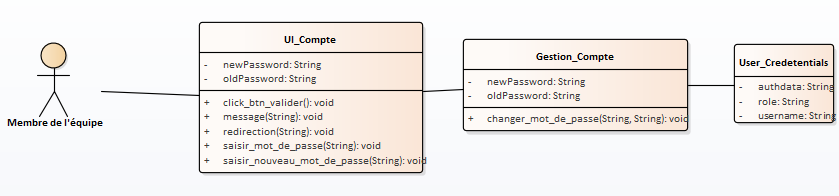
\includegraphics[scale=0.69]{figures/diagrams/class/changepassword_class_diag.png}
 \caption{Diagramme de classes d'analyse de la fonctionnalité "modifier le mot de passe"}
 \label{code77}
\end{figure}

\subsubsection{Consulter le tableau de bord personnel}
La figure \ref{code78} représente le diagramme de classes d'analyse de la fonctionnalité "consulter le tableau de bord personnel".
\begin{figure}[H]
  \centering
 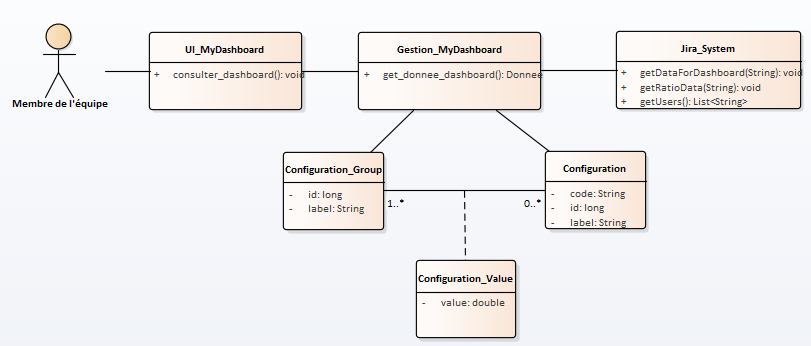
\includegraphics[scale=0.69]{figures/diagrams/class/mydashboard_class_diag.png}
 \caption{Diagramme de classes d'analyse de la fonctionnalité "consulter le tableau de bord personnel"}
 \label{code78}
\end{figure}

\subsubsection{Editer les informations relatives à la planification et consulter le résultat}
La figure \ref{code79} représente le diagramme de classes d'analyse de la fonctionnalité "éditer les informations relatives à la planification et consulter le résultat".
\begin{figure}[H]
  \centering
 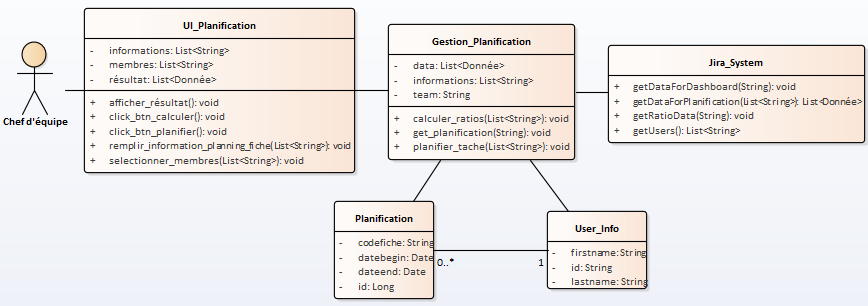
\includegraphics[scale=0.75]{figures/diagrams/class/planification_class_diag.png}
 \caption{Diagramme de classes d'analyse de la fonctionnalité "éditer les informations relatives à la planification et consulter le résultat"}
 \label{code79}
\end{figure}

\subsection{Modélisation dynamique}
%Diagramme de séquences détaillé ou état transition%
Nous présentons dans cette partie la modélisation dynamique de ce sprint sous forme de diagrammes de séquences pour chaque fonctionnalité.

\subsubsection{Modifier le mot de passe}
Pour modifier le mot de passe, le membre de l'équipe doit saisir l'ancien et le nouveau mot de passe. Puis, il valide par le bouton valider. Si le mot de passe est incorrecte, un message d'erreur apparaît. Sinon, un message de validation apparaît pour confirmer le changement.
La figure \ref{code80} représente le diagramme de séquence de la fonctionnalité "modifier le mot de passe".
\begin{figure}[H]
  \centering
 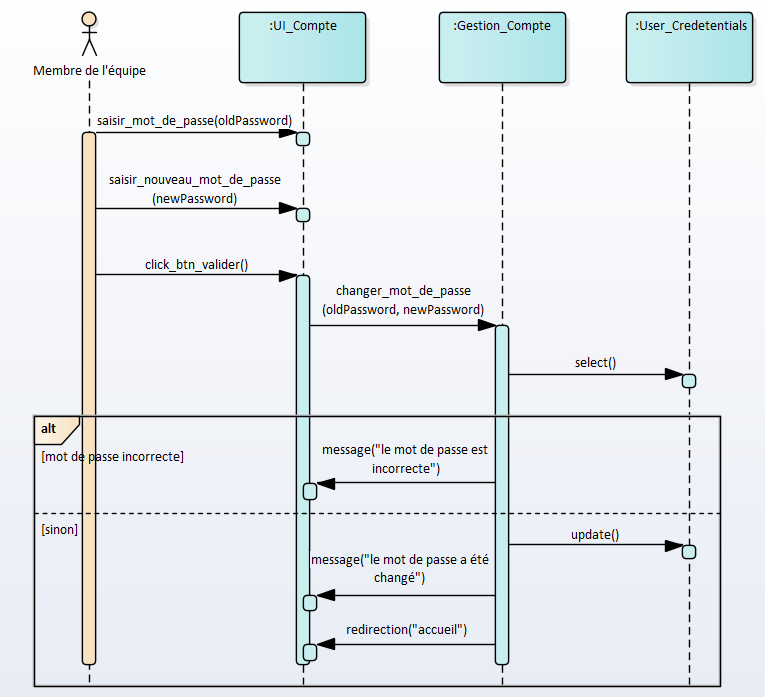
\includegraphics[scale=0.69]{figures/diagrams/sequence/changepassword_seq_diag.png}
 \caption{Diagramme de séquence de la fonctionnalité "modifier le mot de passe"}
 \label{code80}
\end{figure}

\subsubsection{Consulter le tableau de bord personnel}
Pour consulter le tableau de bord personnel, le membre de l'équipe doit cliquer sur le bouton tableau de bord personnel.
La figure \ref{code81} représente le diagramme de séquence de la fonctionnalité "consulter le tableau de bord personnel".
\begin{figure}[H]
  \centering
 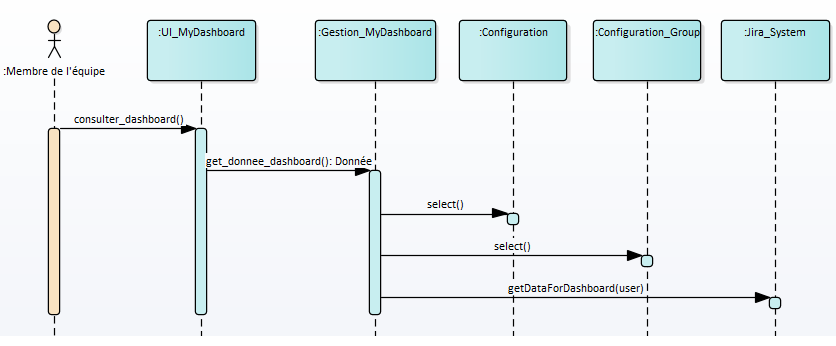
\includegraphics[scale=0.69]{figures/diagrams/sequence/mydashboard_seq_diag.png}
 \caption{Diagramme de séquence de la fonctionnalité "consulter le tableau de bord personnel"}
 \label{code81}
\end{figure}

\subsubsection{Editer les informations relatives à la planification et consulter le résultat}
Pour éditer les informations relatives à la planification et consulter le résultat, le chef d'équipe doit remplir les informations relatives à la fiche. Puis, il clique sur le bouton calculer. Après l'affichage du résultat, le chef d'équipe sélectionne les membres. Et enfin, il clique sur le bouton planifier.
La figure \ref{code82} représente le diagramme de séquence de la fonctionnalité "éditer les informations relatives à la planification et consulter le résultat".
\begin{figure}[H]
  \centering
 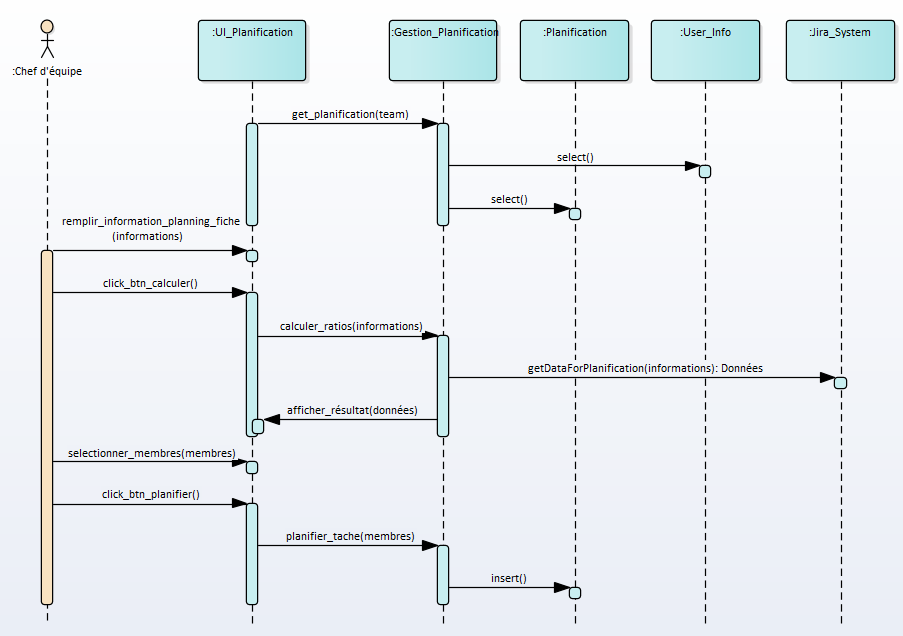
\includegraphics[scale=0.69]{figures/diagrams/sequence/planification_seq_diag.png}
 \caption{Diagramme de séquence de la fonctionnalité "éditer les informations relatives à la planification et consulter le résultat"}
 \label{code82}
\end{figure}

\subsection{Développement du sprint}
%Capture d'écrans%
Le but de cette section est de montrer l'acheminement du sprint en présentant des captures d'écrans des fonctionnalités réalisés dans ce sprint.

\subsubsection{Modifier le mot de passe}
L'utilisateur saisit son ancien mot de passe. Puis il saisit deux fois le nouveau mot de passe et il clique sur le bouton "Enregistrer les modifications". S'il saisit l'ancien mot de passe incorrectement, un message d'erreur apparaît. Sinon, un message de validation de changement de mot de passe apparaît. La figure \ref{code94} représente le message de validation du changement de mot de passe.
\begin{figure}[H]
  \centering
 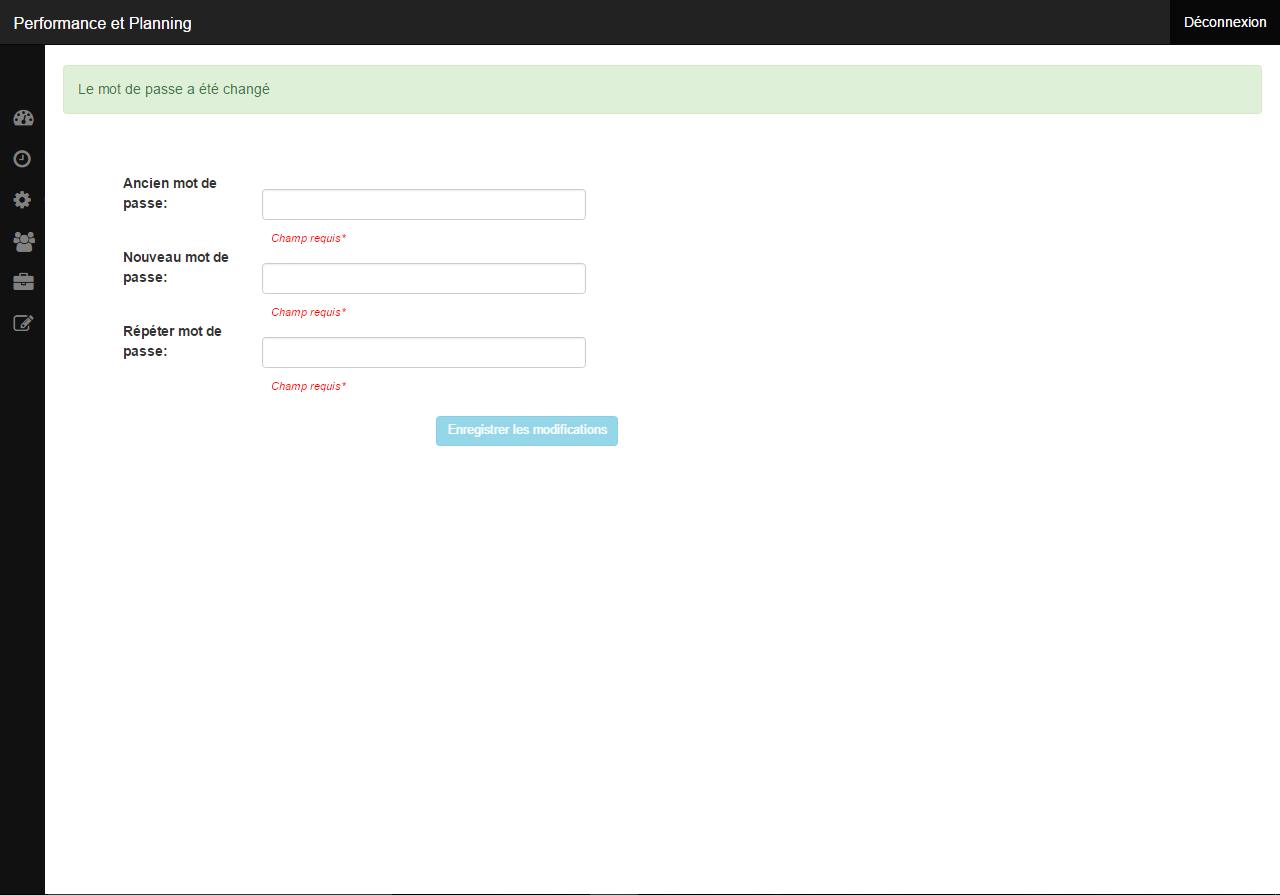
\includegraphics[scale=0.37]{figures/printscreen_app/10_6.PNG}
 \caption{Capture d'écran: modifier le mot de passe}
 \label{code94}
\end{figure}

\subsubsection{Consulter le tableau de bord personnel}
L'utilisateur peut consulter son tableau de bord. Ceci en cliquant sur le bouton tableau de bord du menu vertical situé à gauche. La figure \ref{code95} représente le tableau de bord d'un simple membre.
\begin{figure}[H]
  \centering
 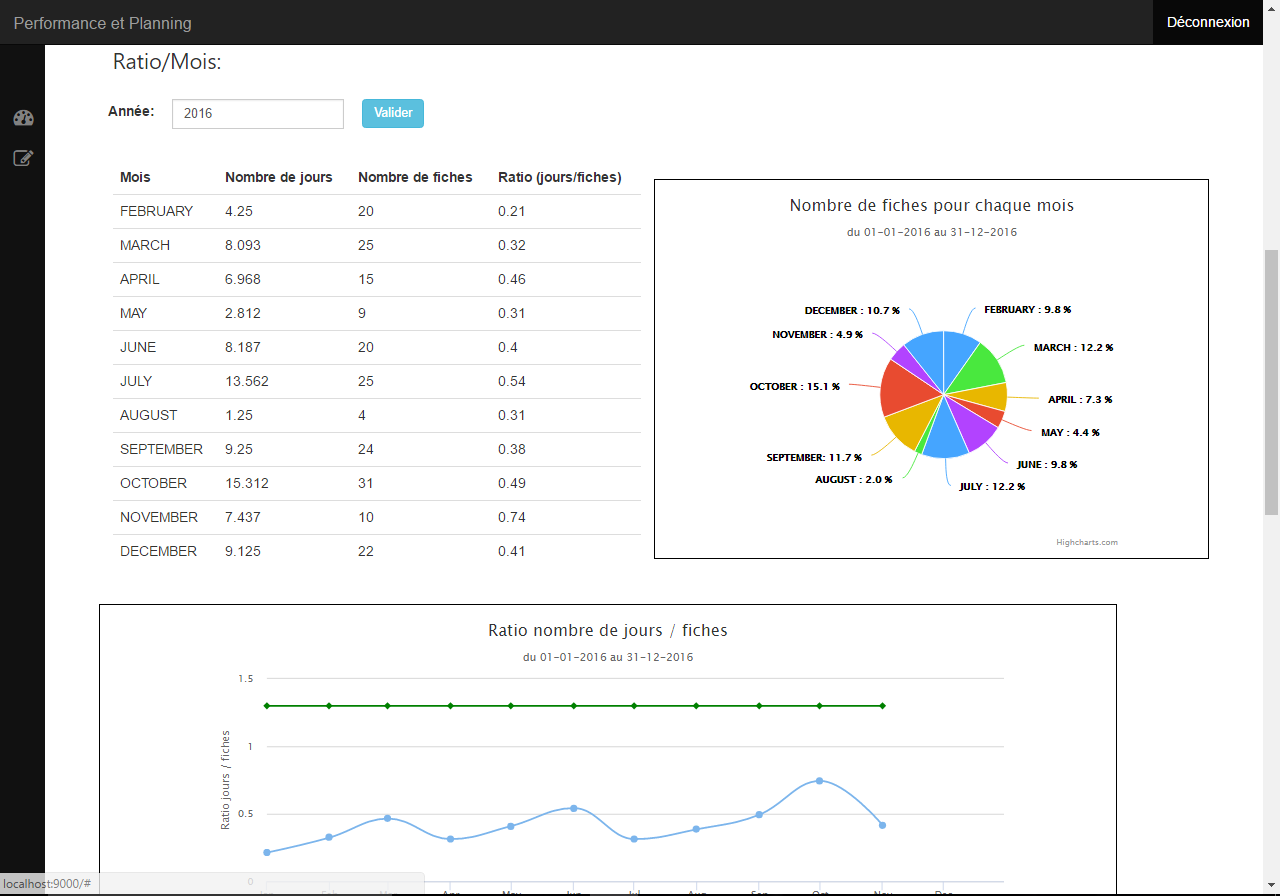
\includegraphics[scale=0.37]{figures/printscreen_app/11_2.PNG}
 \caption{Capture d'écran: consulter le tableau de bord personnel}
 \label{code95}
\end{figure}

\subsubsection{Editer les informations relatives à la planification et consulter le résultat}
L'utilisateur peut rechercher une tâche déjà existante dans la base de données Jira pour remplir les champs de la planification ou les sélectionner lui-même. Il clique après sur le bouton calculer pour avoir la liste des membres de l'équipe et leurs ratios. Il sélectionne ceux qui vont réaliser la tâche et le ratio total s'actualise. Si l'utilisateur clique sur le bouton Valider, la planification est enregistré dans la base de données. La figure \ref{code96} représente le message de validation de la planification.
\begin{figure}[H]
  \centering
 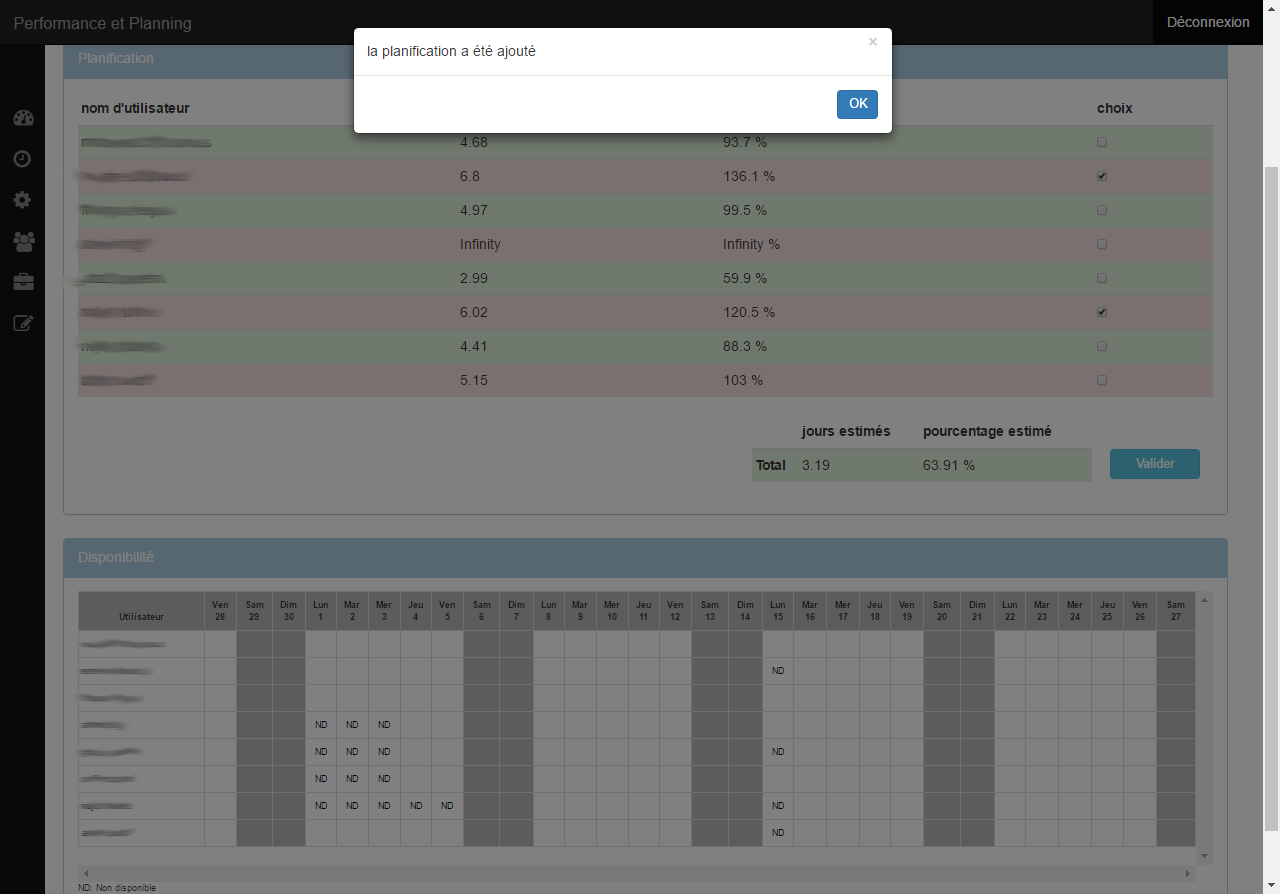
\includegraphics[scale=0.37]{figures/printscreen_app/12_5.PNG}
 \caption{Capture d'écran: éditer les informations relatives à la planification et consulter le résultat}
 \label{code96}
\end{figure}

\subsection{Test et revue du sprint}
%Burndown chart%
Dans cette section, nous allons présenté l’avancement de notre sprint sous forme de burndown chart. La figure \ref{code97} représente la burndown chart de notre sprint.
\begin{figure}[H]
  \centering
 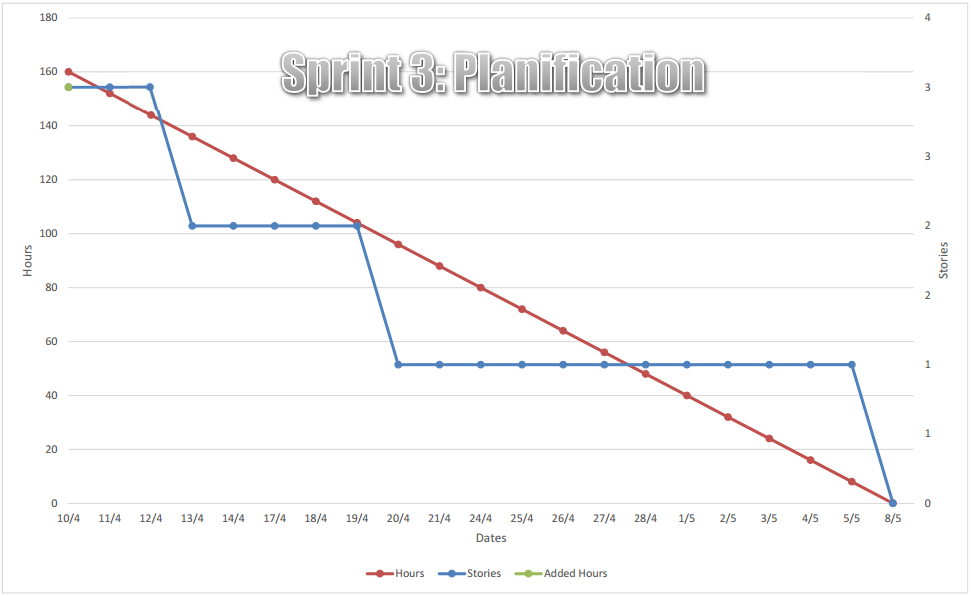
\includegraphics[scale=0.7]{figures/burndown_chart/sprint3.png}
 \caption{Burndown Chart du sprint 3: Planification}
 \label{code97}
\end{figure}

\subsection{Rétrospective}
Cette section est dédiée à l'énumération des problèmes rencontrés dans ce sprint. Ces derniers se résument comme suit:
\begin{itemize}
    \item[$\bullet$] Comprendre les ratios et trouver comment les extraire.
    \item[$\bullet$] Trouver comment calculer le ratio total à partir des ratios des membres sélectionnés.
    \item[$\bullet$] Se familiariser avec la manipulation de dates et ceci sur trois niveaux: AngularJS, Spring et base de données Oracle.
\end{itemize}
\section{Déploiement de l'application}
Dans cette section, nous allons présenter le déploiement de notre application. Cette dernière est composé de deux grands modules qui sont l'application back office qui est accessible via un service web et qui interagit avec nos deux bases de données via le protocole HTTP, et l'application front office qui représente l'interface de communication avec le client. Ces deux modules communiquent entre eux gràce au protocole HTTP. Pour pouvoir déployer notre application nous avons générer en premier lieu un fichier .war pour chaque partie. Puis, nous les avons héberger sur nos deux serveur Tomcat. La figure \ref{code_deploiement_diag} représente le diagramme de déploiement pour notre application.
\begin{figure}[H]
  \centering
 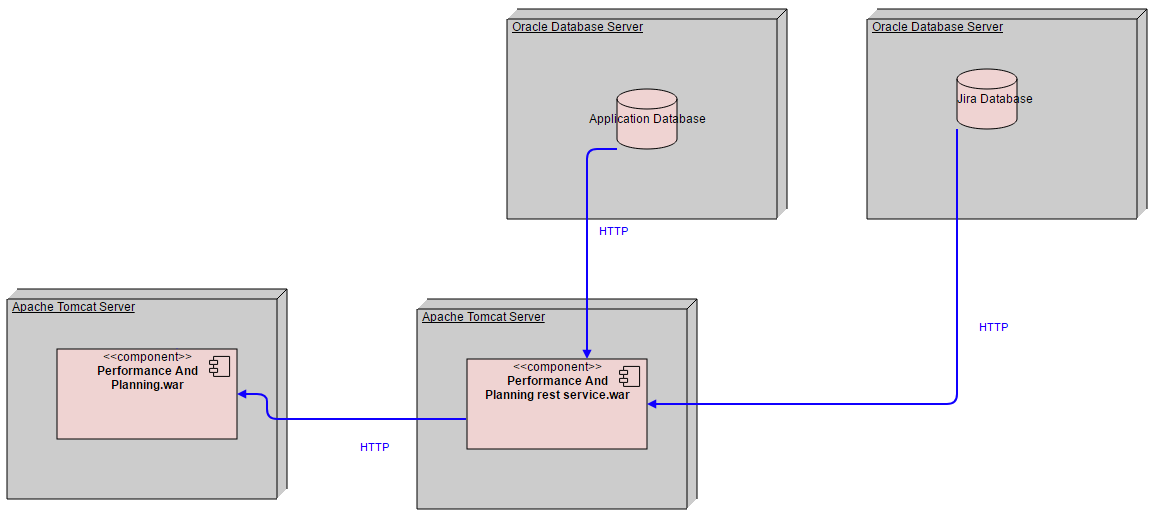
\includegraphics[scale=0.55]{figures/diagrams/Deploiment/deploiment_diag.PNG}
 \caption{Diagramme de déploiement de notre application}
 \label{code_deploiement_diag}
\end{figure}
\section{Conclusion}
Dans ce chapitre, nous avons présenté les sprints de notre projet. En premier lieu, nous avons spécifié le planning pour chaque sprint. Après, nous avons présenté la modélisation statique et dynamique. Ensuite, nous avons détaillé le développement du sprint. Et enfin, nous avons présenté le test, la revue du sprint et la rétrospective.